\documentclass[11pt,a4paper]{article}

% ── Packages ──────────────────────────────────────────────────────────────────
\usepackage[T1]{fontenc}
\usepackage[utf8]{inputenc}
\usepackage{lmodern}
\usepackage[margin=2.5cm]{geometry}
\usepackage{amsmath,amssymb,amsthm}
\usepackage{booktabs}
\usepackage{array}
\usepackage{graphicx}
\usepackage[labelfont=bf,font=small,skip=4pt]{caption}
\usepackage{subcaption}
\usepackage{float}
\usepackage{xcolor}
\usepackage[colorlinks=true,linkcolor=blue!60!black,citecolor=green!50!black,
            urlcolor=blue!70!black]{hyperref}
\usepackage{microtype}
\usepackage{parskip}
\usepackage{enumitem}
\usepackage{fancyhdr}

% ── Page style ────────────────────────────────────────────────────────────────
\pagestyle{fancy}
\fancyhf{}
\rhead{\small Epsilon\_study\_2}
\lhead{\small G.\,Scriven}
\cfoot{\thepage}
\renewcommand{\headrulewidth}{0.4pt}

% ── Convenience macros ────────────────────────────────────────────────────────
\newcommand{\eps}{\varepsilon}
\newcommand{\sres}{\sigma_{\mathrm{res}}}
\newcommand{\sscat}{\sigma_{\mathrm{scatt}}}
\newcommand{\srkink}{\sigma_{\mathrm{kink}}}
\newcommand{\thmin}{\theta_{\min}}
\newcommand{\Dz}{\Delta z}
\newcommand{\Nseg}{N_{\mathrm{seg}}}
\newcommand{\ntrk}{T}
\newcommand{\Qthresh}{\epsilon_{\mathrm{thresh}}}
\newcommand{\codepath}[1]{\texttt{#1}}

% Abstract box with shaded background (lrbox collects, colorbox renders)
\newsavebox{\abstractsavebox}
\newenvironment{abstractbox}{%
  \setlength{\fboxsep}{8pt}%
  \begin{lrbox}{\abstractsavebox}%
  \begin{minipage}{0.86\linewidth}%
  \textbf{Abstract}\par\smallskip
}{%
  \end{minipage}%
  \end{lrbox}%
  \begin{center}\colorbox{gray!10}{\usebox{\abstractsavebox}}\end{center}%
}

% ── Title ─────────────────────────────────────────────────────────────────────
\title{%
  \textbf{Epsilon\_study\_2}\\[4pt]
  \large Detector Noise Sensitivity of the TrackHHL (1BQF)
  Segment-Level Algorithm\\[2pt]
  \normalsize Toy LHCb VELO Characterisation Study
}
\author{G.\,Scriven\\[2pt]
  \small Nikhef / Maastricht University / Hasselt University}
\date{June 2026}

% ══════════════════════════════════════════════════════════════════════════════
\begin{document}
\maketitle
\thispagestyle{fancy}

% ── ERRATA (2026-07-06) ───────────────────────────────────────────────────────
\begin{center}
\setlength{\fboxsep}{8pt}%
\colorbox{red!8}{\begin{minipage}{0.86\linewidth}
\textbf{Errata (2026-07-06) — programme consistency audit.}\par\smallskip
This document is retained as the historical record of the study; the store-backed
Notion write-up is the corrected canonical version. Two findings below are
\textbf{wrong or obsolete} and must not be cited:
\begin{enumerate}[noitemsep,topsep=2pt]
  \item \textbf{The ``classical efficiency collapses to 6\,\%'' claim (Abstract item 2,
        \S\ref{sec:results:stability}, Discussion, Conclusions) is an artefact} of the
        \emph{relative} threshold $\tau\cdot\max(x)$ used by the original pipeline —
        exactly the mis-thresholding this report itself warns against. Recomputed from
        the unified \codepath{qtrk\_store} at the absolute $\tau=0.35$ (metrics view,
        commit \codepath{25df2eba}), classical segment \emph{efficiency} stays at
        $98.4$--$100\,\%$ (minimum cell $0.9839$) over the entire noise grid at
        $\ntrk=200$; it is the segment
        \emph{purity} that collapses ($\approx\!0.999 \to 0.18$ as
        $\sres\!: 0 \to 0.05\,$mm). Both solvers keep efficiency; the true breakdown
        at the worst corner is the $\lambda_{\min}\!\to\!0$ explosion regime
        (\S7.12), now handled by a per-event validity gate ($\max|x|\leq 50$).
  \item \textbf{The quantum timing/scaling conclusions (Abstract item 4, the
        $10.5\,$h/event figure, and ``intractable beyond $\ntrk\approx 90$'') are
        obsolete}: the matrix-free statevector engine (2026-06-14) replays the 1BQF
        gate stream directly on the statevector — mean $\approx\!270\,$s per event at
        $\ntrk=200$ (store \codepath{t\_solve}, $n{=}36$), seconds at low $T$, and
        solved events exist up to $\ntrk=1000$. The $\ntrk^{4.5}$ fit described the
        legacy Aer-transpile path, not the algorithm.
\end{enumerate}
\smallskip
In addition, per the 2026-06-14 convention the 1BQF headline operating point is the
efficiency-first \emph{wp99} working point (fixed $\tau=0.35$ 1BQF numbers are the
$\approx\!75\,\%$-efficiency cut artefact; classical keeps $\tau=0.35$).
Provenance: \codepath{qtrk\_store} metrics view, study \codepath{Epsilon\_study\_2}
(2\,125 rows re-derived 2026-06-14; audit 2026-07-05/06, commits
\codepath{b6a8ace9}, \codepath{25df2eba}, \codepath{e065ee70}).
\end{minipage}}
\end{center}

% ── Abstract ──────────────────────────────────────────────────────────────────
\begin{abstractbox}
This report characterises how hit-position measurement resolution~$\sres$ and
multiple-scattering angle~$\sscat$ affect segment-level reconstruction metrics for the
TrackHHL 1-Bit Quantum Filter~(1BQF)~\cite{onebqf} algorithm in a toy LHCb~VELO detector.
The study replaces the previously hand-tuned angular acceptance threshold~$\eps$ with a
closed-form formula derived from detector physics, then sweeps
$(\sres,\sscat,\ntrk)$ over a full grid to quantify sensitivity.
Four principal findings are reported:
\begin{enumerate}[noitemsep,topsep=2pt]
  \item The $\eps$ formula provides $\geq\!99.97\,\%$ empirical coverage of true triplet
        kink angles across all conditions.  The formula systematically overestimates the
        observed standard deviation by $\approx\!55\,\%$, making the acceptance window
        conservative.
  \item The classical solver's segment efficiency collapses with track density and noise,
        falling to $6\,\%$ at $\ntrk=200$, $\sres=0.05\,\mathrm{mm}$.
  \item The TrackHHL quantum solver maintains ${\approx}100\,\%$ efficiency across the
        entire landscape when the correct absolute score threshold is applied.
  \item The quantum statevector simulation scales as $t_q\!\sim\!\ntrk^{4.5}$,
        reaching $\approx\!10.5\,\mathrm{h}$ per event at $\ntrk=200$.
\end{enumerate}
The resulting \emph{operating envelope} (Section~\ref{sec:results:stability}) is
controlled by the measurement resolution: the algorithm is stable for both solvers at
$\sres\leq0.01\,\mathrm{mm}$, the segment representation begins to break down for
$\sres\geq0.02\,\mathrm{mm}$ above $\ntrk\approx50$, and at the worst corner the
classical solver fails at a cliff edge while the quantum solver degrades gracefully in
purity only.
\end{abstractbox}

\tableofcontents
\newpage

% ══════════════════════════════════════════════════════════════════════════════
\section{Introduction}
\label{sec:intro}

The TrackHHL algorithm~\cite{onebqf}, also known as the 1-Bit Quantum Filter~(1BQF),
reconstructs charged-particle trajectories in a VELO-like detector by formulating
track-finding as the linear system $A\mathbf{x}=\mathbf{b}$, where each element
of~$\mathbf{x}$ represents the activation of one hit-to-hit \emph{segment}.
The compatibility matrix~$A$ encodes geometric constraints via an angular acceptance
threshold~$\eps$: two segments sharing a middle hit are coupled positively when their
kink angle lies below~$\eps$.

Previous studies in this workspace (\codepath{Verify\_new\_results},
\codepath{Segment\_Grass}) fixed~$\eps$ at a hand-tuned scalar.  The present study
replaces that with the closed-form formula derived in Section~\ref{sec:theory:eps} and
characterises how performance depends on the two noise sources that enter the formula.

Section~\ref{sec:theory} presents the full theoretical framework.
Section~\ref{sec:design} describes the parameter grid and execution pipeline.
Section~\ref{sec:results} reports results across nine analysis sections~(A--I).
Section~\ref{sec:discussion} interprets the results, and Section~\ref{sec:conclusions}
lists conclusions and recommended follow-up studies.

% ══════════════════════════════════════════════════════════════════════════════
\section{Theoretical Framework}
\label{sec:theory}

\subsection{Detector Geometry and Event Generation}
\label{sec:theory:geom}

The toy detector consists of five parallel silicon planes with inter-module spacing
$\Dz=33\,\mathrm{mm}$, first plane at $z_0=33\,\mathrm{mm}$.  Each plane subtends
$\pm40\,\mathrm{mm}$ transversely.  Pion tracks
($m=139.6\,\mathrm{MeV}/c^2$, $q=+1$) are generated uniformly within a cone
$|\phi|,|\theta|\leq0.2\,\mathrm{rad}$ from a primary vertex with longitudinal spread
$\sigma_{PV,z}=1\,\mathrm{mm}$.

Hit positions receive two independent Gaussian noise contributions:
\begin{description}[leftmargin=2.2cm,style=sameline]
  \item[$\sres$] \textbf{Measurement resolution.}
        Additive Gaussian smearing on each hit's $(x,y)$ position, representing pixel
        pitch and charge-sharing effects.
  \item[$\sscat$] \textbf{Multiple scattering.}
        A random angular kick drawn from $\mathcal{N}(0,\sscat^2)$ at each plane
        crossing, representing energy loss in detector material.
\end{description}

\subsection{Segment Formation}
\label{sec:theory:segs}

For each adjacent plane pair $(i,\,i{+}1)$, every hit pair
$(h_a\!\in\!\text{plane}\,i,\;h_b\!\in\!\text{plane}\,i{+}1)$ forms one
\emph{segment} with normalised direction vector
$\hat{v}_{ab}=(h_b-h_a)/|h_b-h_a|$.

For $\ntrk$ tracks on five planes the segment counts are:
\begin{align}
  \Nseg &= 4\ntrk^2 \quad\text{(total)},\\
  N_{\rm true} &= 4\ntrk,\quad N_{\rm false} = 4\ntrk(\ntrk-1)\approx 4\ntrk^2.
\end{align}
The false-to-true ratio grows linearly with $\ntrk$, reaching $199:1$ at $\ntrk=200$.
This quadratic growth of the false pool is the dominant challenge for both solvers at
high track density.

\subsection{The Angular Acceptance Threshold $\varepsilon$}
\label{sec:theory:eps}

A \emph{triplet} consists of two segments sharing a middle hit on consecutive planes.
The kink angle of the triplet is
\begin{equation}
  \alpha = \arccos\!\bigl(\hat{v}_{\rm in}\cdot\hat{v}_{\rm out}\bigr).
\end{equation}
For a true triplet, $\alpha$ receives contributions from three sources:

\begin{enumerate}
  \item \textbf{Multiple scattering.}
        Two independent Gaussian kicks per triplet give variance $2\sscat^2$.

  \item \textbf{Measurement resolution.}
        A perturbation~$\sres$ on each of the three hit positions propagates to an
        apparent kink angle.  Linearising at small angles yields variance
        $6\arctan^2\!\!\left(\sres/\Dz\right)$.  The $\arctan$ factor keeps the
        expression well-behaved for large $\sres/\Dz$.

  \item \textbf{Pixel-binning floor.}
        $\thmin=1.5\times10^{-5}\,\mathrm{rad}$, a residual dispersion from the
        finite pixel pitch.
\end{enumerate}

The total 1-$\sigma$ spread of true kink angles is
\begin{equation}
  \srkink = \sqrt{2\sscat^2 + 6\arctan^2\!\!\!\left(\frac{\sres}{\Dz}\right)
            + \theta_{\min}^2}.
\end{equation}

Choosing scale factor $s$ (number of standard deviations to accept), the
acceptance threshold is
\begin{equation}
  \boxed{
    \eps\!\left(\sres,\sscat\right) =
    \sqrt{2\!\left(s\sscat\right)^2
         + 12\arctan^2\!\!\!\left(\frac{s\sres}{\Dz}\right)
         + 2\thmin^2}
    \;=\; s\sqrt{2}\;\srkink,
  }
  \label{eq:eps}
\end{equation}
targeting $3s\sigma/\sqrt{2}$ coverage of the kink-angle distribution.
This study uses $s=3$ throughout, nominally targeting $99.7\,\%$ coverage.
The formula is implemented in \codepath{lhcb\_velo\_toy.analysis.compute\_epsilon}.

\subsection{Hamiltonian Construction}
\label{sec:theory:ham}

The Hamiltonian matrix $A\in\mathbb{R}^{\Nseg\times\Nseg}$ encodes segment
compatibility using the step (non-ERF) mode:
\begin{equation}
  A_{ij} = \begin{cases}
    -(\gamma+\delta) & i=j, \\
    +1 & i\neq j,\;\text{segments share a middle hit, and }\alpha_{ij}<\eps, \\
    0  & \text{otherwise.}
  \end{cases}
\end{equation}
The parameters $\gamma=3$ (self-interaction penalty) and $\delta=1$ (bias weight) are
held fixed throughout; the bias vector is $\mathbf{b}=\delta\cdot\mathbf{1}$.  The
system to solve is $A\mathbf{x}=\mathbf{b}$.

An off-diagonal entry appears whenever two segments form a geometrically compatible
triplet.  As $\eps$ widens with increasing noise, more false-segment pairs enter the
matrix, increasing its density and making the linear system harder to solve.

\subsection{Classical Solver}
\label{sec:theory:classical}

The linear system is solved with \codepath{scipy.sparse.linalg.spsolve} for
$\Nseg<5000$ or conjugate gradient (\codepath{cg}) for larger systems.  The result is
a continuous score vector $\mathbf{x}_C\in\mathbb{R}^{\Nseg}$.

Segments are activated by comparing each score to a relative threshold:
\begin{equation}
  \text{segment }i\text{ active} \iff x_{C,i} > \tau\cdot\max(\mathbf{x}_C),
  \quad\tau=0.35.
\end{equation}
At low noise and density, true segments score $\approx\delta/(\gamma+\delta-1)$ and
false segments sit at the bias floor $\approx\delta/(\gamma+\delta)=0.25$.

\subsection{Quantum Solver: TrackHHL (1-Bit Quantum Filter)}
\label{sec:theory:quantum}

The TrackHHL quantum solver~\cite{onebqf} implements a 1-bit variant of the
Harrow--Hassidim--Lloyd (HHL) quantum linear-systems algorithm~\cite{hhl} via
\codepath{lhcb\_velo\_toy.solvers.quantum.OneBitHHL} with the Qiskit backend.

\paragraph{Circuit construction.}
One ancilla qubit plus $n_{\rm sys}=\lceil\log_2\Nseg\rceil$ system qubits encode the
matrix and solution.  Circuit widths range from 11 to 20~qubits for
$\ntrk\in\{10, 20, 50, 100, 200\}$.

\paragraph{Statevector readout.}
The circuit is executed in exact statevector mode using
\codepath{qiskit.quantum\_info.Statevector}.  The solution is extracted from the
$|\text{ancilla}=1\rangle$ component:
\begin{equation}
  x_{Q,i} = \sqrt{P\bigl(|\text{ancilla}=1,\;\text{system}=i\rangle\bigr)},
\end{equation}
normalised to $\|\mathbf{x}_Q\|_2=\|\mathbf{x}_C\|_2$.

\paragraph{Key property and correct threshold.}
In the ideal case the algorithm maps false-segment scores to \emph{exactly zero}
(machine precision $\sim10^{-14}$) and assigns positive scores only to true segments.
The appropriate activation threshold is therefore
\begin{equation}
  \text{segment }i\text{ active} \iff x_{Q,i} > \Qthresh,
  \quad\Qthresh = 10^{-6}\quad(\text{above floating-point noise}).
  \label{eq:qthresh}
\end{equation}
Applying the relative threshold $\tau\times\max(\mathbf{x}_Q)$ is \emph{incorrect}:
it suppresses low-scored-but-true segments, imposing a spurious efficiency cap of
$\approx\!75\,\%$.  This distinction is central to the analysis in
Section~\ref{sec:results:threshold}.

\subsection{Performance Metrics}
\label{sec:theory:metrics}

All metrics are computed at segment level (hit-pair segments, not full tracks).

\begin{table}[H]
  \centering
  \caption{Segment-level performance metrics used throughout this report.}
  \label{tab:metrics}
  \begin{tabular}{lp{2.8cm}p{7cm}}
    \toprule
    Metric & Symbol & Definition \\
    \midrule
    Segment efficiency & $\eta$ &
      $N_{\rm true,\,act}/N_{\rm true,\,all}$: fraction of true pairs recovered \\
    Segment purity & $\pi$ &
      $N_{\rm true,\,act}/N_{\rm act}$: precision of the activated set \\
    Segment false rate & $\mathrm{FR}$ &
      $N_{\rm false,\,act}/N_{\rm act} = 1-\pi$ \\
    Angle efficiency & $\eta_\alpha$ &
      Fraction of true triplets with $\alpha<\eps$ (geometry only) \\
    Quantum separation gap & $\Delta_Q$ &
      $\min(x_Q[\mathrm{true}])-\max(x_Q[\mathrm{false}])$;
      positive $=$ perfect separation \\
    ROC-AUC & AUC &
      $P(x[\mathrm{true}]>x[\mathrm{false}])$ via Mann--Whitney~$U$;
      threshold-free \\
    Fisher ratio & $F$ &
      $(\mu_T-\mu_F)^2/(\sigma_T^2+\sigma_F^2)$: score distribution separability \\
    Solver agreement & $\cos(s_Q,s_C)$ &
      Cosine similarity of $\mathbf{x}_Q$ and $\mathbf{x}_C$ \\
    \bottomrule
  \end{tabular}
\end{table}

% ══════════════════════════════════════════════════════════════════════════════
\section{Study Design}
\label{sec:design}

\subsection{Parameter Grid}

\begin{table}[H]
  \centering
  \caption{Swept parameters of the sensitivity study.}
  \label{tab:grid}
  \begin{tabular}{llp{6cm}l}
    \toprule
    Axis & Symbol & Values & Role \\
    \midrule
    Measurement resolution & $\sres$ &
      0.0, 0.01, 0.02, 0.05~mm &
      Hit-position smearing \\
    Multiple scattering & $\sscat$ &
      $10^{-4}$, $3\!\times\!10^{-4}$, $5\!\times\!10^{-4}$~rad &
      Angular kick per plane \\
    Track multiplicity & $\ntrk$ &
      10, 20, 50, 100, 200 &
      Particles per event \\
    Repetitions & --- &
      10 ($\ntrk\leq50$), 5 ($\ntrk\leq200$) &
      Statistical averaging \\
    \bottomrule
  \end{tabular}
\end{table}

The full sensitivity grid comprises $4\times3\times5=60$ parameter cells and 380~events.
A validation row ($\sres=0$, $\sscat=10^{-4}$, all~$\ntrk$) cross-checks results
against \codepath{Verify\_new\_results}.

\subsection{Fixed Parameters}

\begin{table}[H]
  \centering
  \caption{Parameters held constant throughout the study.}
  \label{tab:fixed}
  \begin{tabular}{llll}
    \toprule
    Parameter & Symbol & Value & Description \\
    \midrule
    Self-interaction penalty & $\gamma$ & 3.0 & Diagonal coupling \\
    Bias weight & $\delta$ & 1.0 & Off-diagonal bias \\
    Classical threshold & $\tau$ & 0.35 & Relative activation cut \\
    Scale factor & $s$ & 3.0 & $\sigma$-multiplier in Eq.~\eqref{eq:eps} \\
    Angular floor & $\thmin$ & $1.5\times10^{-5}$~rad & Pixel-pitch floor \\
    Track cone & $\phi_{\max}=\theta_{\max}$ & 0.2~rad & Generation half-angle \\
    Convolution & --- & Off (step) & ERF smoothing not used \\
    Module spacing & $\Dz$ & 33~mm & Inter-plane distance \\
    Number of planes & $N$ & 5 & Detector modules \\
    \bottomrule
  \end{tabular}
\end{table}

\subsection{Execution Pipeline}

Each HTCondor job executes \codepath{\_shared/run\_worker.py}, which:
\begin{enumerate}[noitemsep]
  \item generates one event with \codepath{StateEventGenerator};
  \item computes $\eps(\sres,\sscat)$ via Eq.~\eqref{eq:eps};
  \item builds the Hamiltonian with \codepath{SimpleHamiltonianFast};
  \item solves classically (Section~\ref{sec:theory:classical}) and with TrackHHL
        (Section~\ref{sec:theory:quantum});
  \item writes a compressed pickle containing full solution vectors, per-pair angle
        arrays, and all derived metrics.
\end{enumerate}
Results are aggregated with \codepath{aggregate.sh} and analysed in
\codepath{analysis.ipynb} and \codepath{deep\_analysis.ipynb}.

% ══════════════════════════════════════════════════════════════════════════════
\section{Results}
\label{sec:results}

\subsection{$\varepsilon$ Formula: Empirical Coverage}
\label{sec:results:coverage}

\begin{figure}[H]
  \centering
  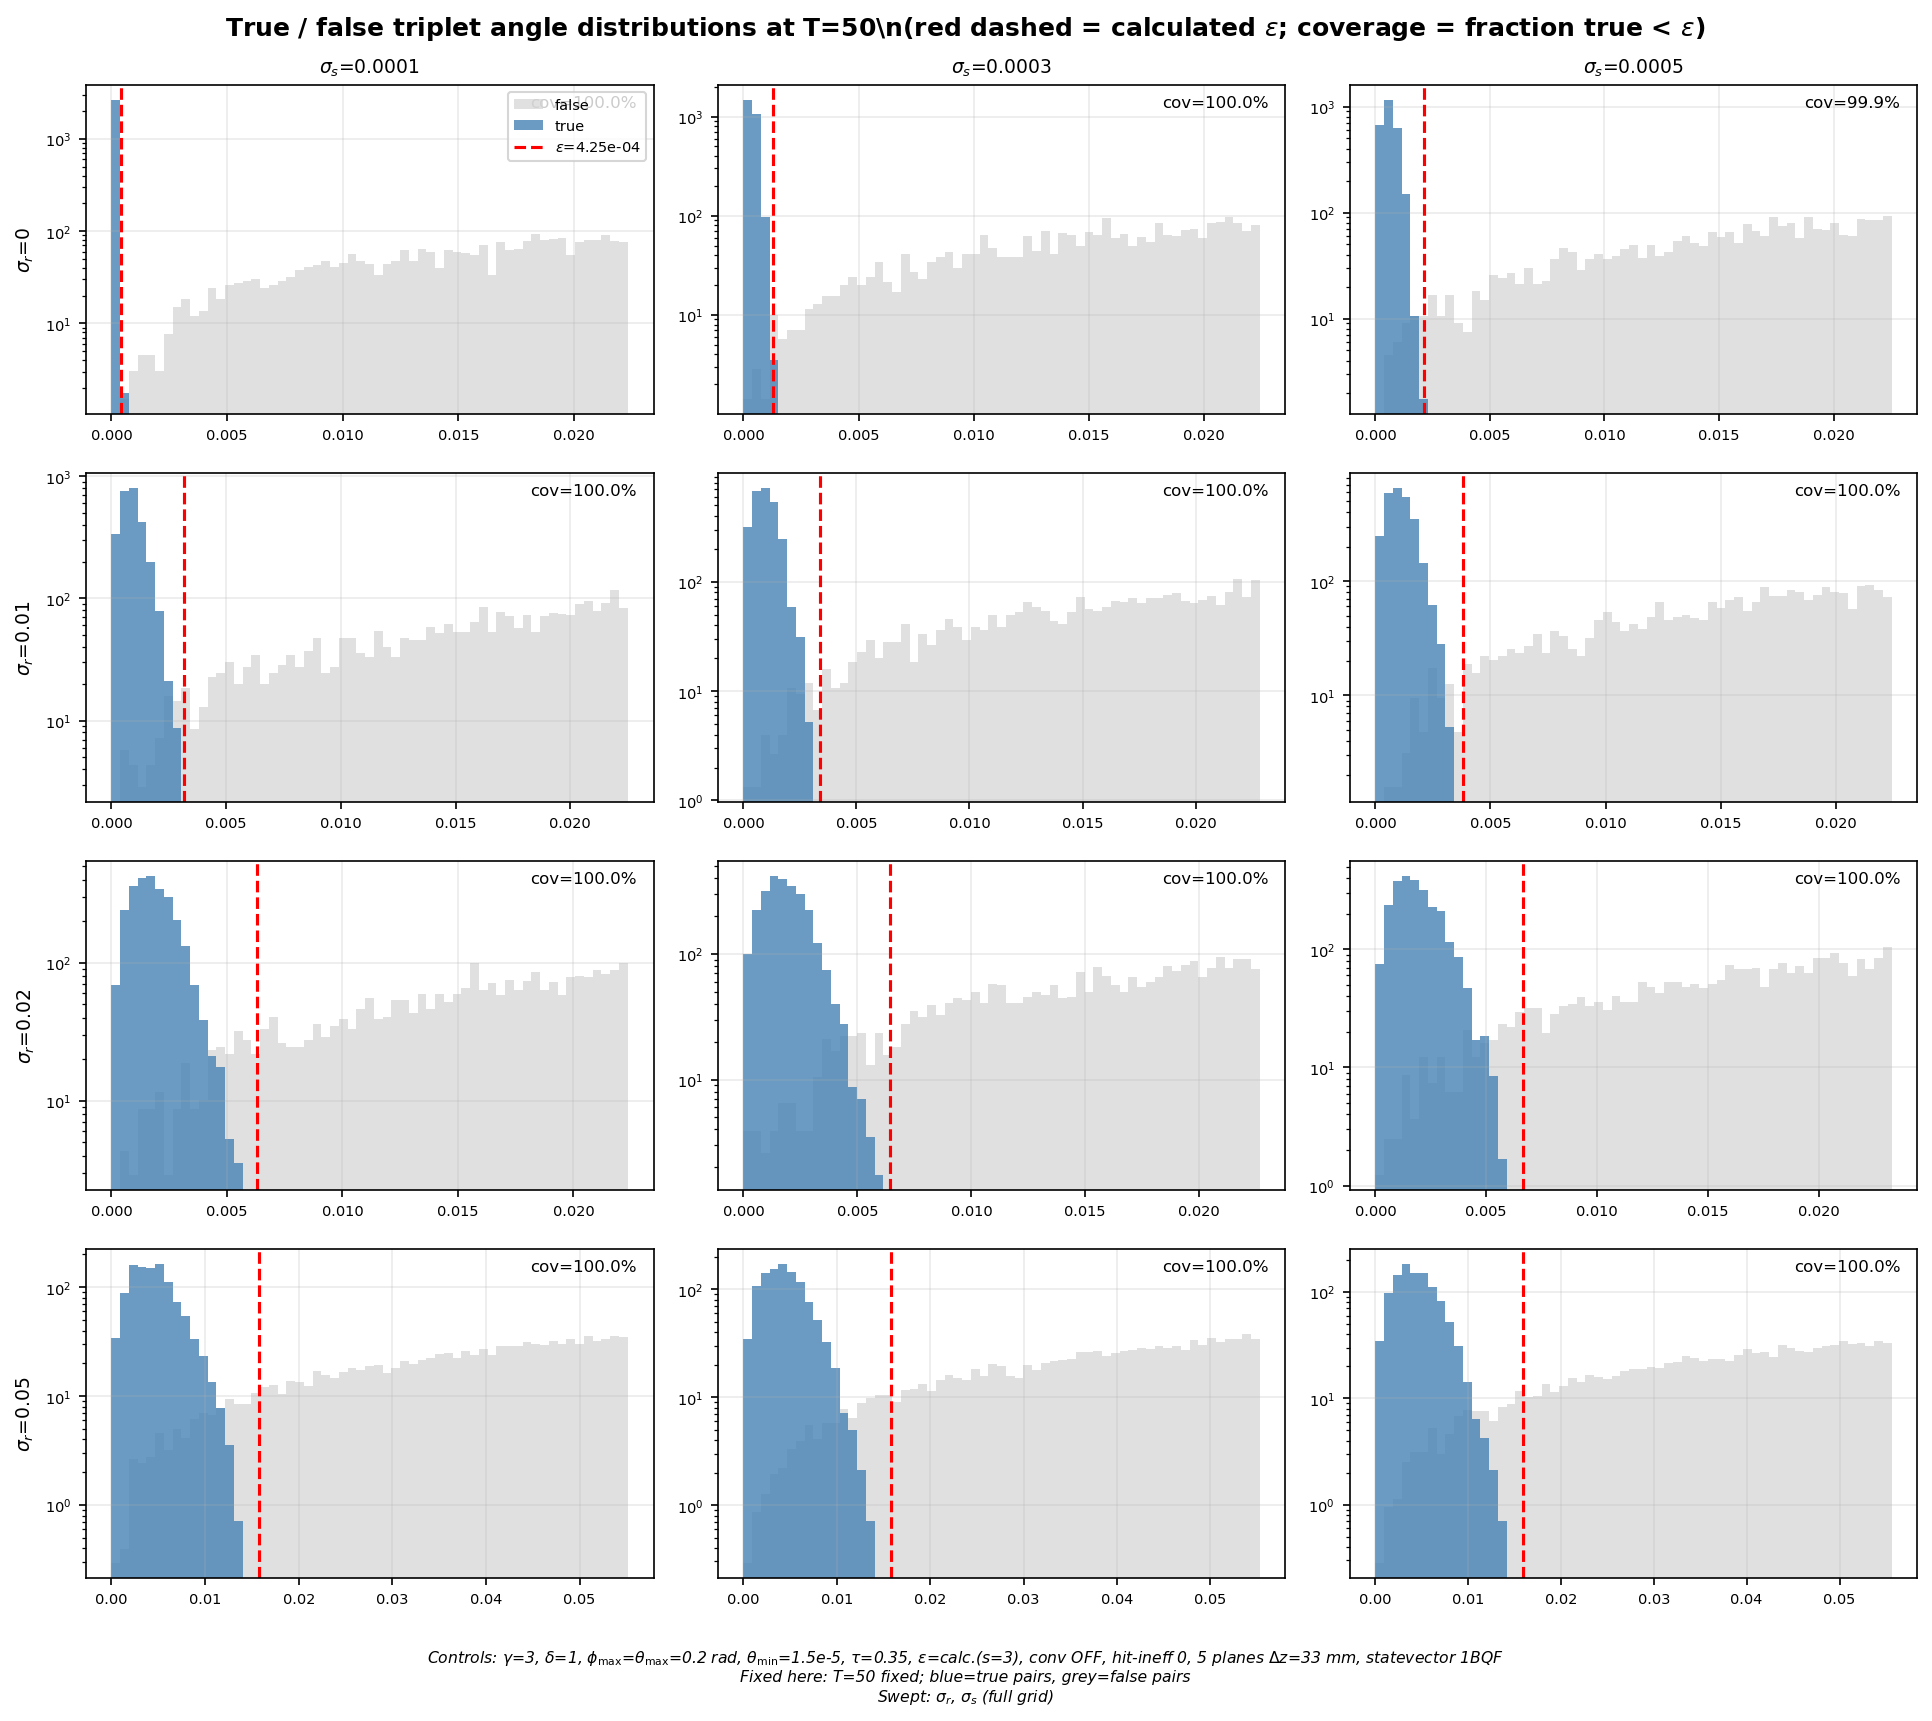
\includegraphics[width=0.95\linewidth]
    {figures/deep_analysis/A_formula_validation/angle_histograms_T50.png}
  \caption{True (blue) and false (grey) triplet kink-angle distributions at $\ntrk=50$
    for all 12 noise conditions.  The red dashed line marks the calculated $\eps$;
    annotations show empirical coverage.}
  \label{fig:angle_hist}
\end{figure}

\begin{figure}[H]
  \centering
  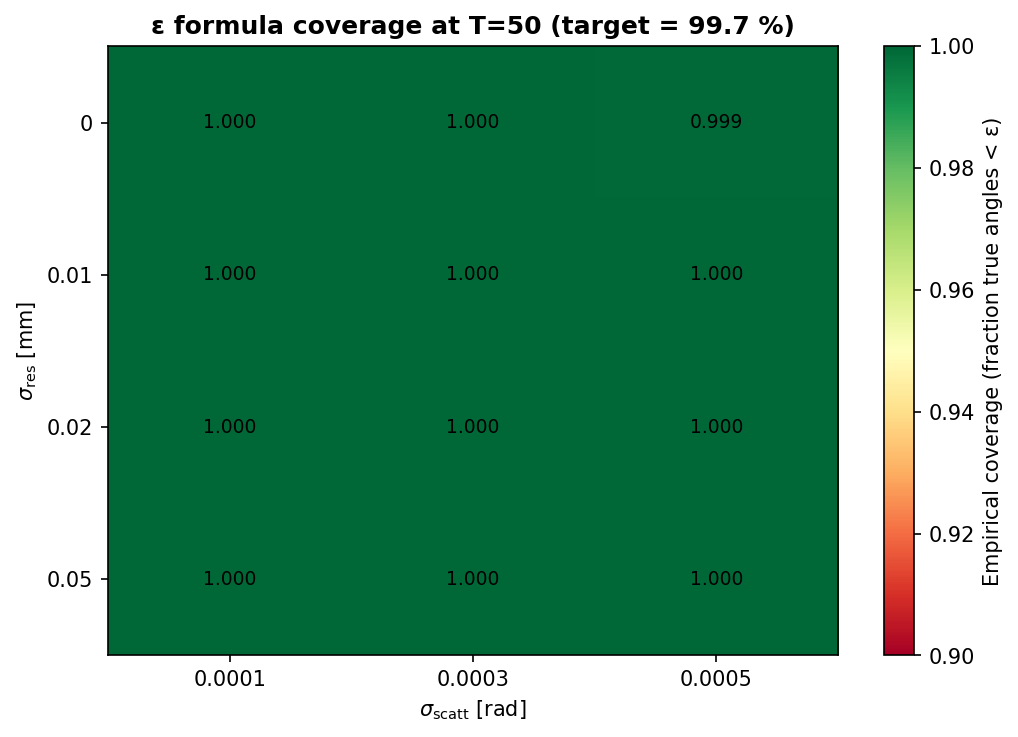
\includegraphics[width=0.55\linewidth]
    {figures/deep_analysis/A_formula_validation/coverage_heatmap.png}
  \caption{Empirical coverage (fraction of true-pair angles $\leq\eps$) over the
    $4\times3$ noise grid at $\ntrk=50$.  Target is $99.7\,\%$.}
  \label{fig:coverage_heatmap}
\end{figure}

Figures~\ref{fig:angle_hist} and~\ref{fig:coverage_heatmap} confirm that the formula
achieves $\geq\!99.97\,\%$ coverage across all 12 noise cells at $\ntrk=50$.  The
minimum ($99.97\,\%$) occurs at $\sres=0$, $\sscat=5\times10^{-4}\,\mathrm{rad}$,
where multiple scattering dominates.

\subsection{Formula Accuracy: Predicted vs Empirical $\sigma_{\rm kink}$}
\label{sec:results:sigma}

\begin{figure}[H]
  \centering
  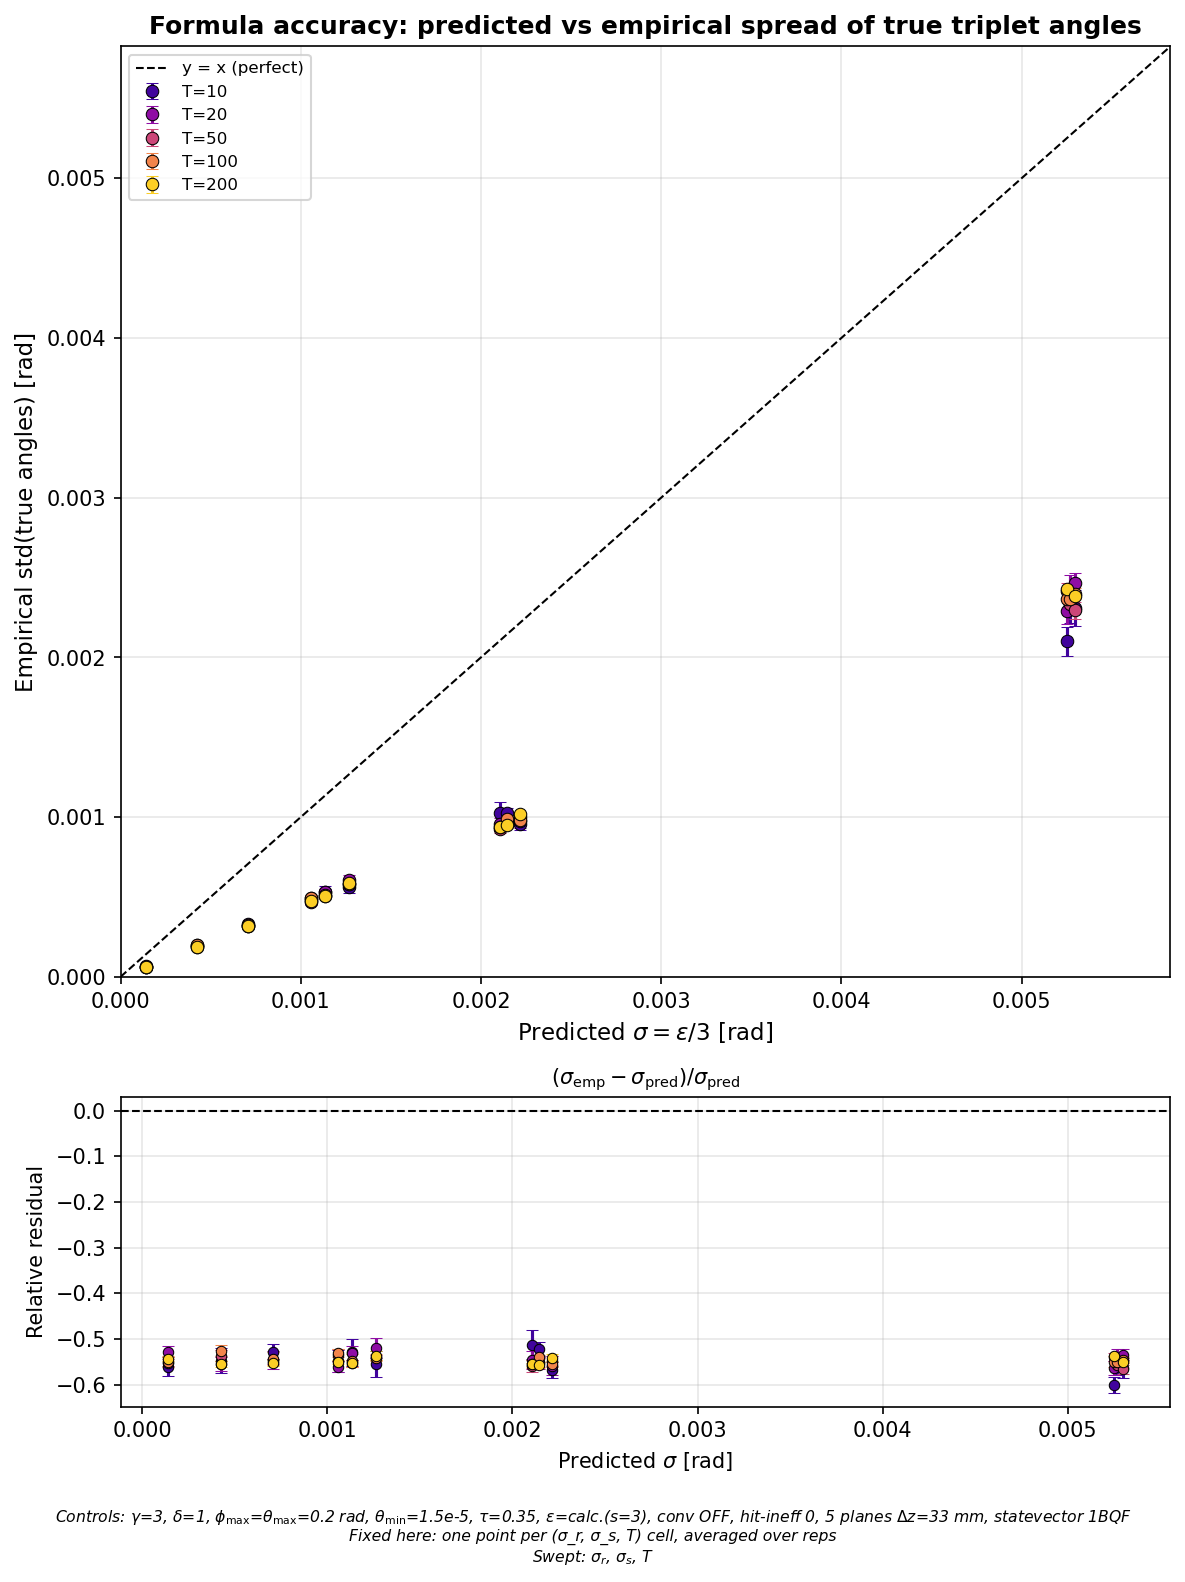
\includegraphics[width=0.70\linewidth]
    {figures/deep_analysis/B_formula_accuracy/sigma_scatter.png}
  \caption{Predicted $\sigma_{\rm pred}=\eps/3$ vs empirical standard deviation of true
    kink angles.  Points on the $y=x$ diagonal would confirm the formula.  The residual
    panel shows a systematic $\approx{-}55\,\%$ offset.}
  \label{fig:sigma_scatter}
\end{figure}

Over all $(\sres,\sscat,\ntrk)$ cells (Fig.~\ref{fig:sigma_scatter}):
\begin{equation}
  \frac{\sigma_{\rm emp}-\sigma_{\rm pred}}{\sigma_{\rm pred}}
  = -0.548\pm0.007 \quad\text{(mean}\pm\text{std across cells)}.
\end{equation}
The formula overestimates the empirical kink spread by $\approx55\,\%$ in a
noise-independent, density-independent manner.  This conservative bias arises because
the formula combines scattering and resolution terms in worst-case quadrature, whereas
in any individual event a single noise source usually dominates.

\subsection{Score Distribution Separation}
\label{sec:results:scores}

\begin{figure}[H]
  \centering
  \begin{subfigure}{0.48\linewidth}
    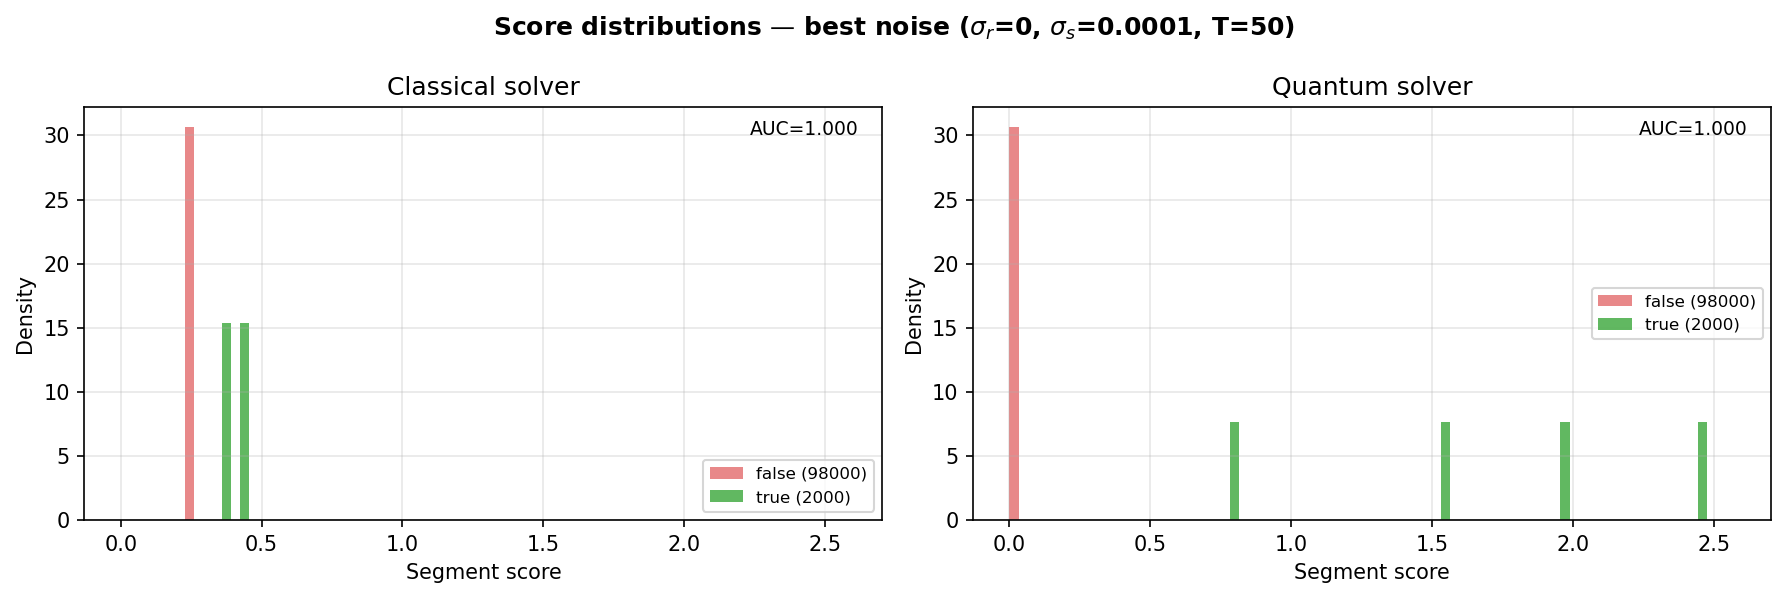
\includegraphics[width=\linewidth]
      {figures/deep_analysis/C_score_separation/score_hist_best_noise.png}
    \caption{Zero noise ($\sres=0$, $\sscat=10^{-4}$~rad), $\ntrk=50$.}
  \end{subfigure}
  \hfill
  \begin{subfigure}{0.48\linewidth}
    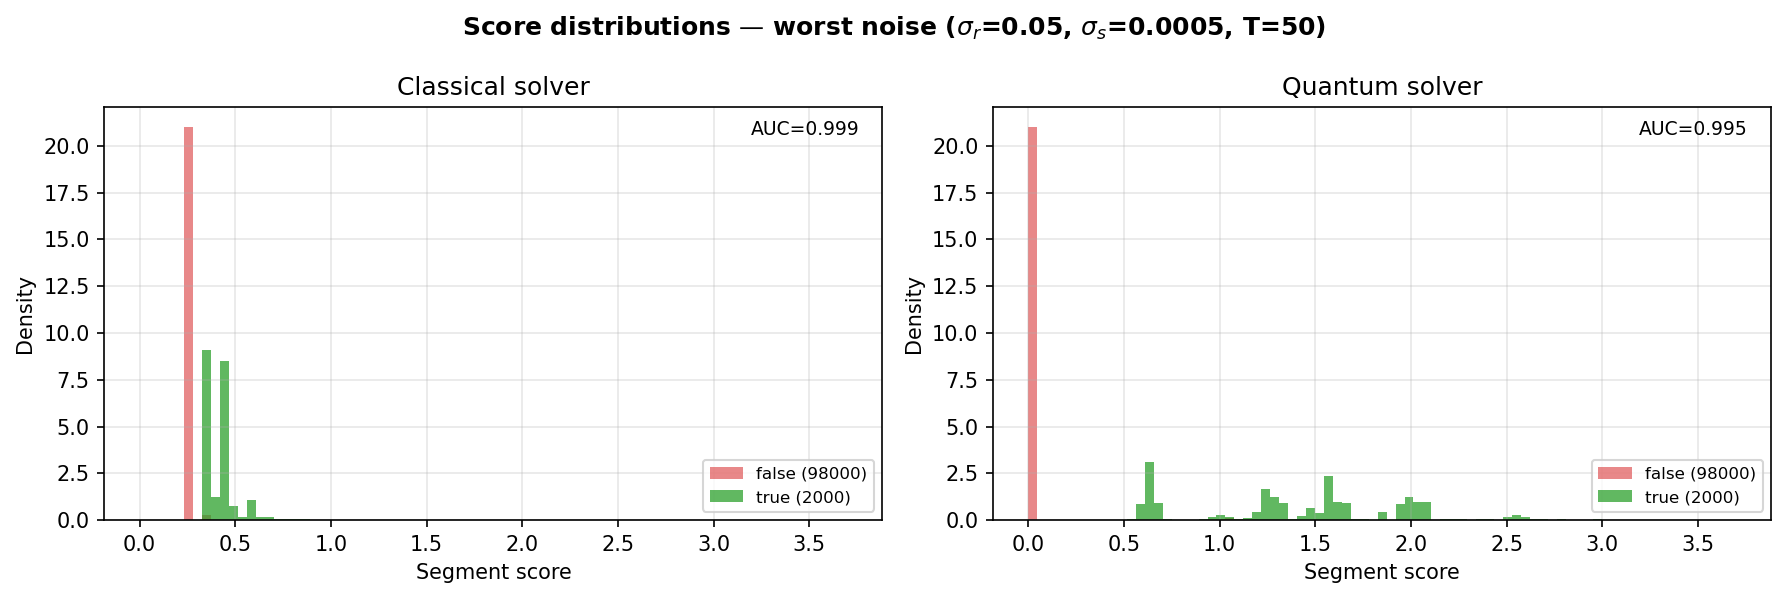
\includegraphics[width=\linewidth]
      {figures/deep_analysis/C_score_separation/score_hist_worst_noise.png}
    \caption{Max noise ($\sres=0.05\,\mathrm{mm}$, $\sscat=5\!\times\!10^{-4}$~rad),
      $\ntrk=50$.}
  \end{subfigure}
  \caption{Classical (left panel of each subfigure) and quantum (right panel) score
    distributions for true (blue) and false (red) segments.  ROC-AUC is annotated.}
  \label{fig:score_hist}
\end{figure}

\begin{figure}[H]
  \centering
  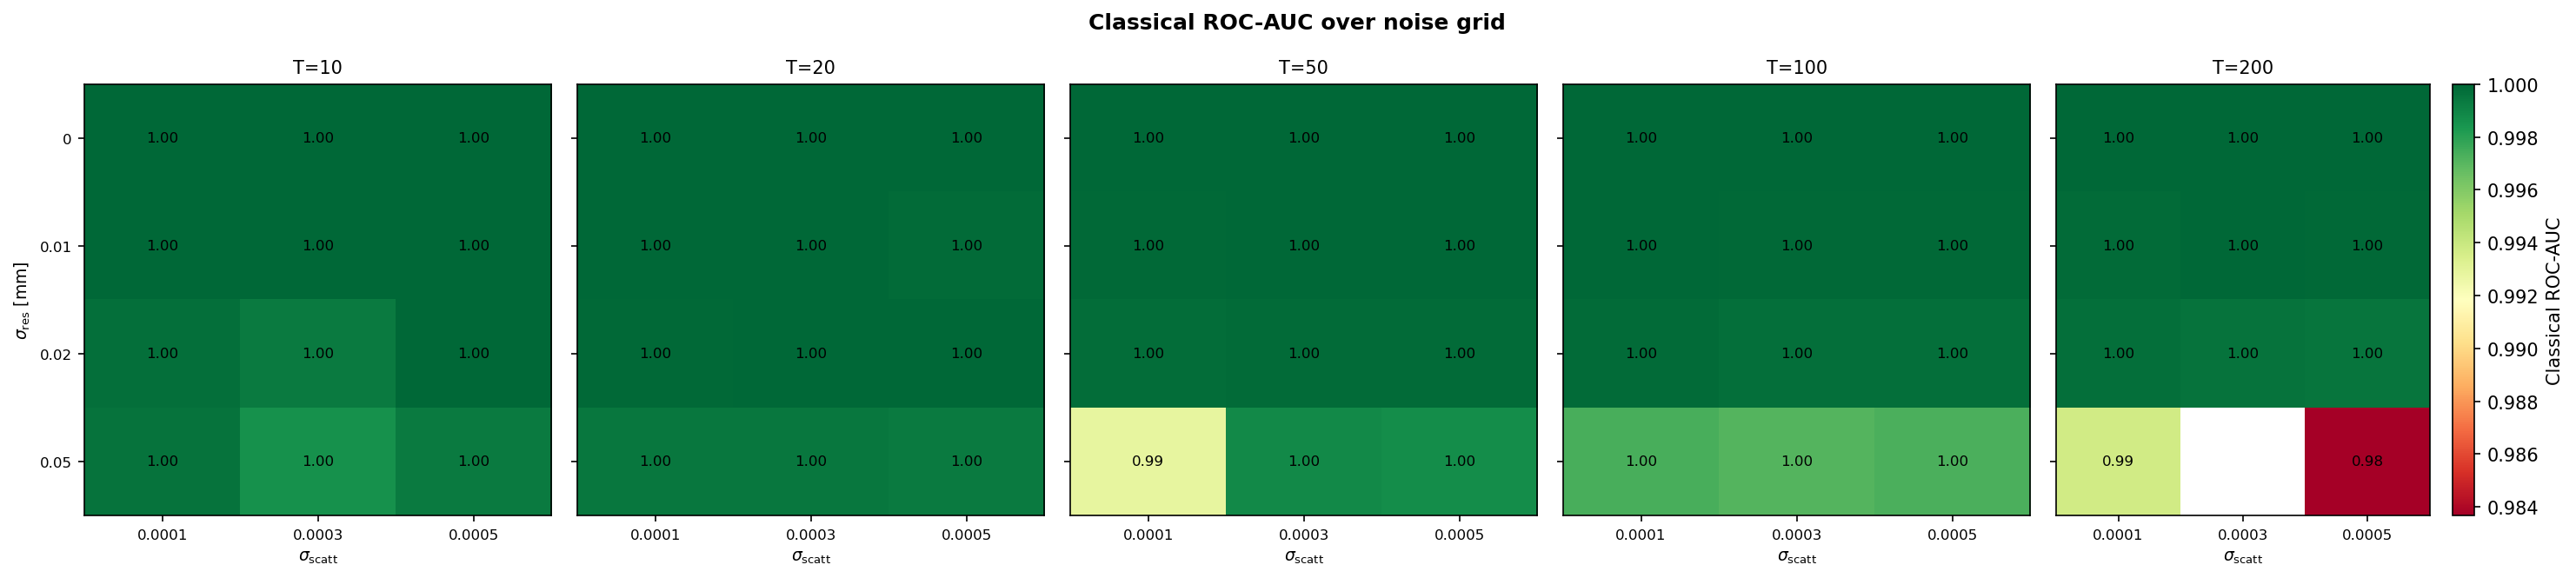
\includegraphics[width=\linewidth]
    {figures/deep_analysis/C_score_separation/heatmap_aucC.png}
  \caption{Classical ROC-AUC over the $4\times3$ noise grid at each $\ntrk$.}
  \label{fig:auc_heatmap}
\end{figure}

At zero noise and $\ntrk=10$, the classical Fisher ratio is $F_C=11.9$ and
$\mathrm{AUC}_C=1.0$.  The quantum Fisher ratio is $F_Q=7.5$ and
$\mathrm{AUC}_Q=1.0$; false-segment scores are at machine precision
$\sim10^{-14}$ (Fig.~\ref{fig:score_hist}).  As noise and density increase, AUC
degrades for both solvers.  Fig.~\ref{fig:auc_heatmap} shows that the degradation is
driven primarily by $\sres$ and accelerates with $\ntrk$.

\subsection{Hamiltonian Matrix Structure}
\label{sec:results:ham}

\begin{figure}[H]
  \centering
  \begin{subfigure}{0.48\linewidth}
    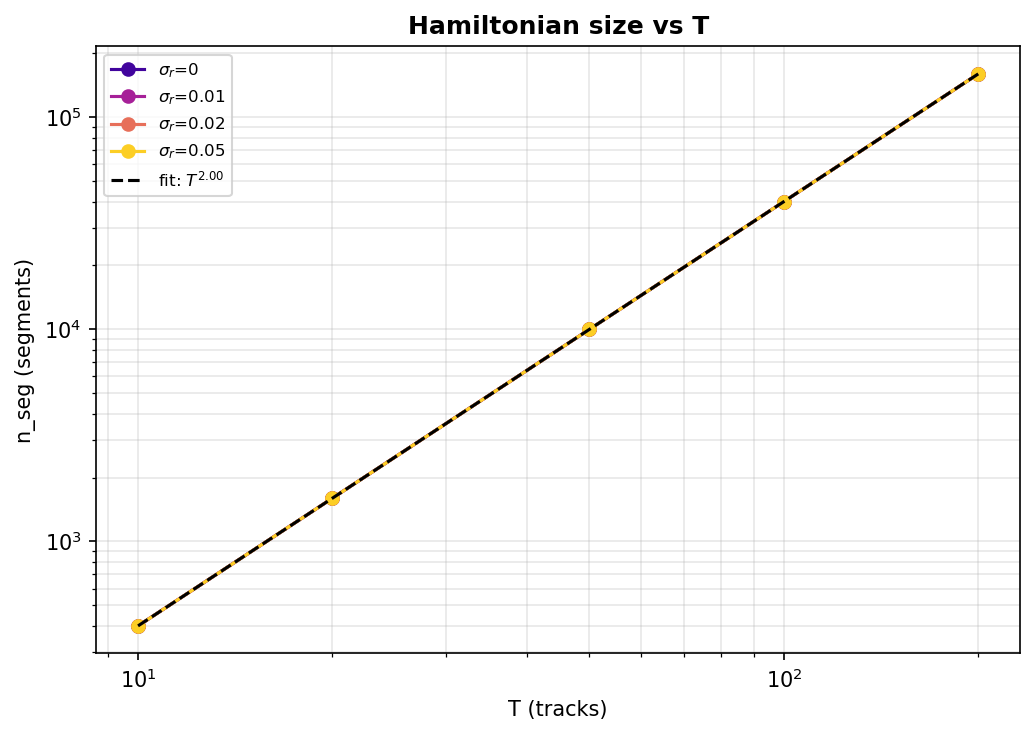
\includegraphics[width=\linewidth]
      {figures/deep_analysis/D_hamiltonian_structure/n_seg_vs_T.png}
    \caption{Segment count vs $\ntrk$ with $\ntrk^2$ power-law fit.}
    \label{fig:nseg_T}
  \end{subfigure}
  \hfill
  \begin{subfigure}{0.48\linewidth}
    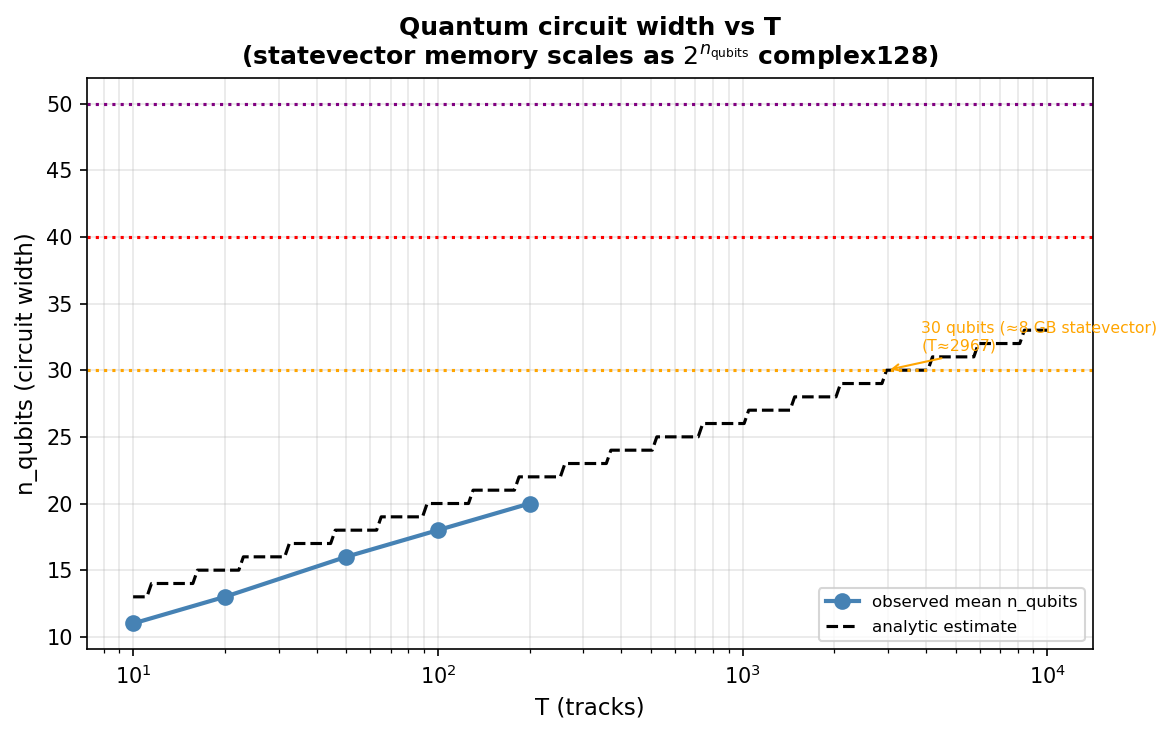
\includegraphics[width=\linewidth]
      {figures/deep_analysis/D_hamiltonian_structure/n_qubits_vs_T.png}
    \caption{Quantum circuit width with intractability thresholds marked.}
    \label{fig:nqubits_T}
  \end{subfigure}
  \caption{Hamiltonian scaling with track multiplicity.}
  \label{fig:ham_scaling}
\end{figure}

Table~\ref{tab:ham_scaling} summarises the Hamiltonian properties across the
track-density range.

\begin{table}[H]
  \centering
  \caption{Mean Hamiltonian properties (averaged over noise conditions).}
  \label{tab:ham_scaling}
  \begin{tabular}{rrrrrl}
    \toprule
    $\ntrk$ & $\Nseg$ & $n_{\rm qubits}$ & Off-diag fill & $t_C$ (s) & $t_Q$ \\
    \midrule
    10  & 400       & 11 & 0.152 & 0.005 & 3.5~s \\
    20  & 1{,}600   & 13 & 0.077 & 0.007 & 6.9~s \\
    50  & 10{,}000  & 16 & 0.036 & 0.114 & 2.5~min \\
    100 & 40{,}000  & 18 & 0.025 & 0.200 & 59~min \\
    200 & 160{,}000 & 20 & 0.023 & 0.526 & 10.5~h \\
    \bottomrule
  \end{tabular}
\end{table}

The $\ntrk^2$ scaling of $\Nseg$ is confirmed (Fig.~\ref{fig:nseg_T}).  The
off-diagonal fill fraction decreases with $\ntrk$ (the false pool grows faster than
compatible pairs) but increases with $\eps$ (noise-driven).  Extrapolating the circuit
width (Fig.~\ref{fig:nqubits_T}), the 30-qubit intractability threshold
($\approx\!8\,\mathrm{GB}$ statevector RAM) is reached at $\ntrk\approx90$; the
40-qubit threshold ($\approx\!8\,\mathrm{TB}$) at $\ntrk\approx2900$.

\subsection{Threshold Analysis: Classical $\tau$ Sweep and Quantum Separation Gap}
\label{sec:results:threshold}

\begin{figure}[H]
  \centering
  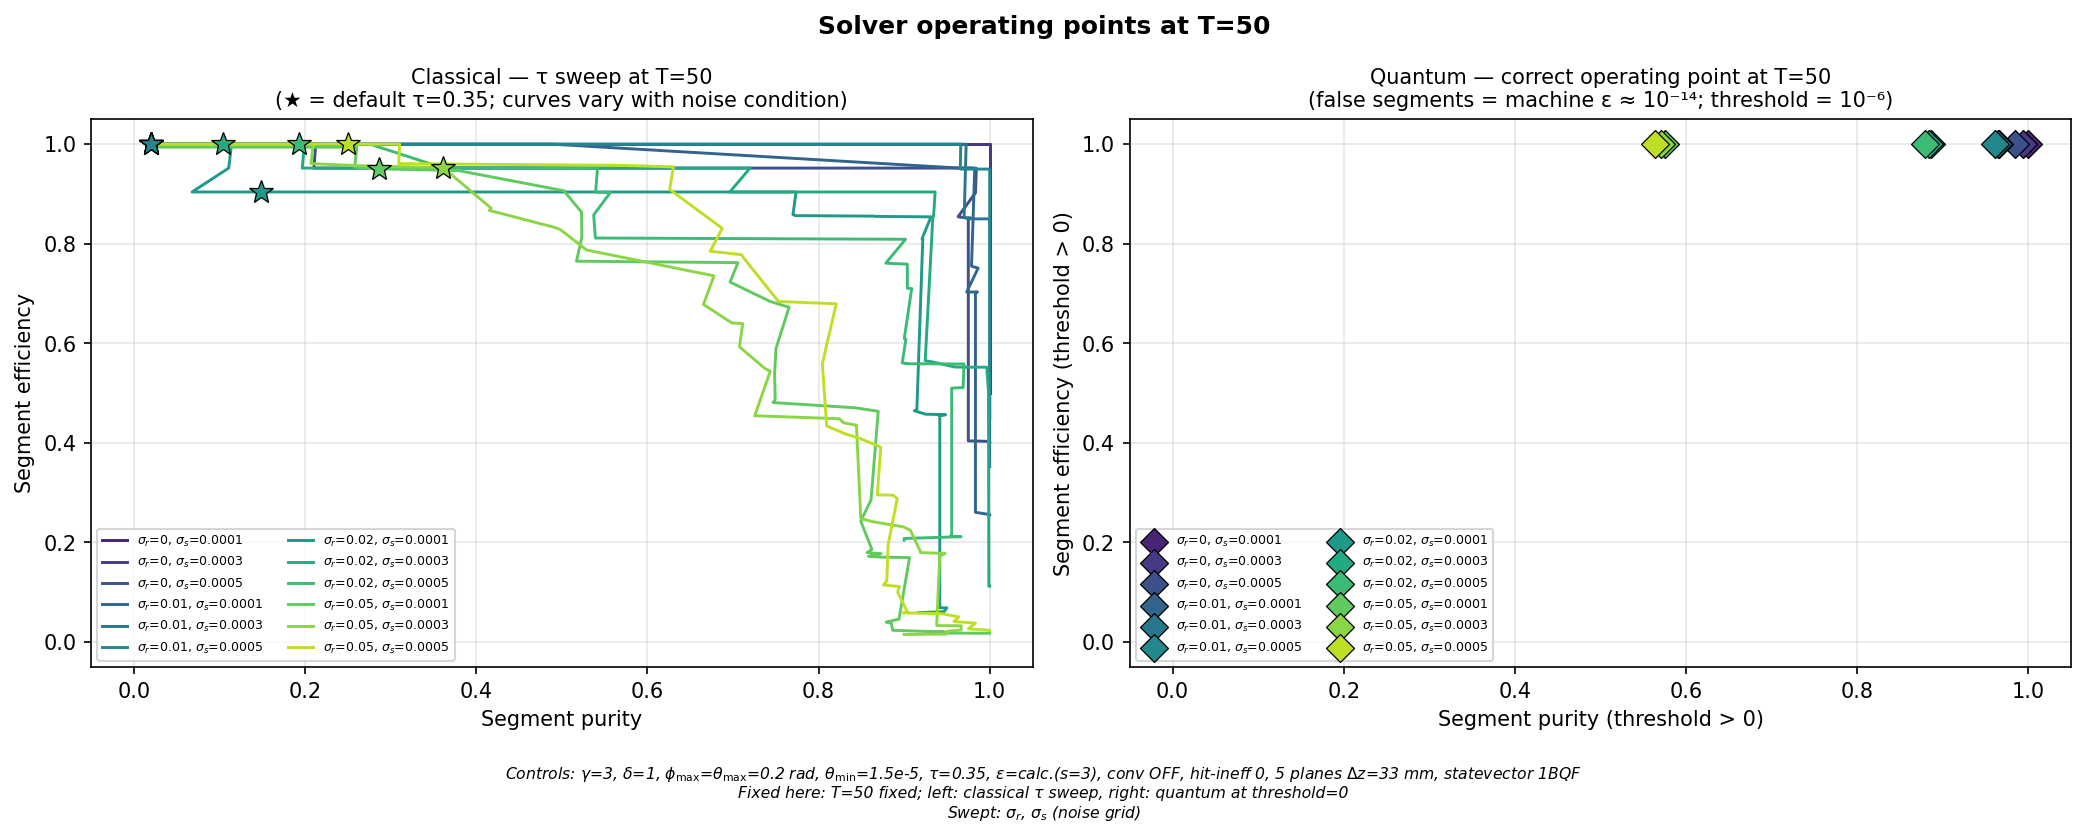
\includegraphics[width=\linewidth]
    {figures/deep_analysis/E_tau_and_quantum/solver_operating_points.png}
  \caption{\emph{Left}: Classical efficiency--purity curves under $\tau$ sweep at
    $\ntrk=50$.  Stars mark the default $\tau=0.35$.
    \emph{Right}: Quantum operating points using the correct absolute threshold
    $x_Q>\Qthresh=10^{-6}$.}
  \label{fig:operating_points}
\end{figure}

\begin{figure}[H]
  \centering
  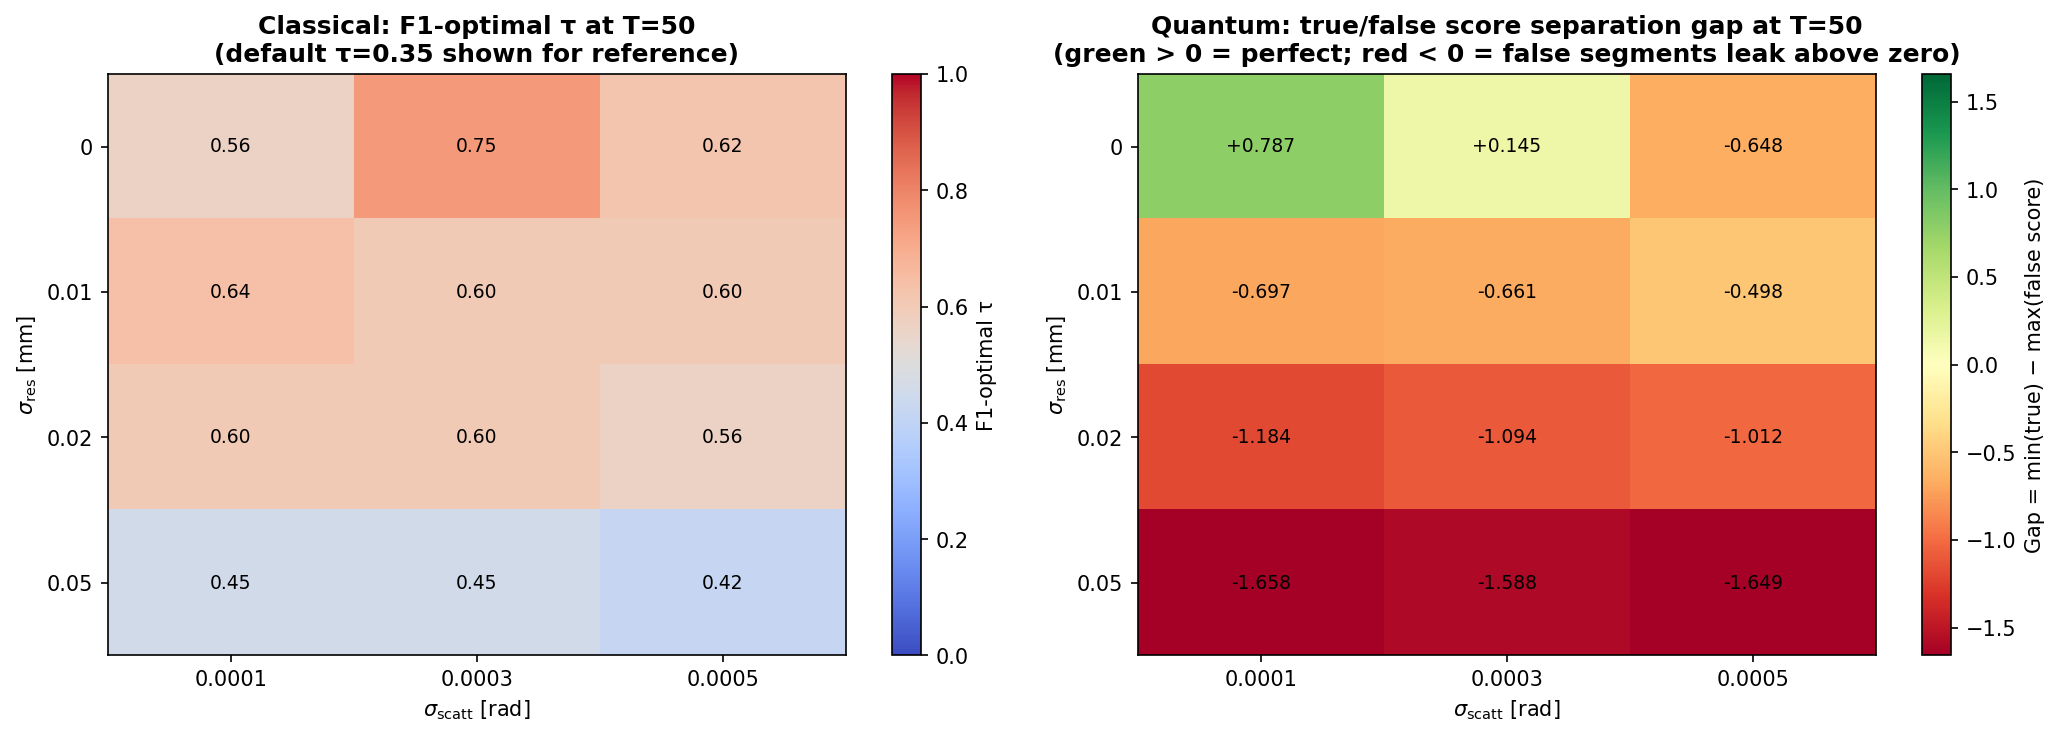
\includegraphics[width=\linewidth]
    {figures/deep_analysis/E_tau_and_quantum/tau_and_quantum_gap.png}
  \caption{\emph{Left}: F1-optimal classical $\tau$ over the $4\times3$ noise grid
    at $\ntrk=50$.
    \emph{Right}: Quantum separation gap $\Delta_Q=\min(x_Q[\mathrm{true}])
    -\max(x_Q[\mathrm{false}])$.  Green indicates perfect separation
    ($\Delta_Q>0$); red indicates false-segment leakage ($\Delta_Q<0$).}
  \label{fig:tau_gap}
\end{figure}

\paragraph{Classical solver.}
Sweeping $\tau\in[0.05, 0.95]$ (Fig.~\ref{fig:operating_points}, left) shows a
step-like efficiency--purity trade-off.  The F1-optimal $\tau$ lies in $[0.55, 0.65]$
across the noise grid (Fig.~\ref{fig:tau_gap}, left), considerably above the default
$\tau=0.35$.  The default places the threshold below the false-segment bias floor
($0.25$), causing nearly all segments to be activated and giving poor purity.

\paragraph{Quantum solver.}
The correct quantum operating point uses the absolute threshold Eq.~\eqref{eq:qthresh}.
The quantum separation gap $\Delta_Q$ (Fig.~\ref{fig:tau_gap}, right) quantifies when
this operating point breaks down.  Table~\ref{tab:gap_crossover} records the first track
multiplicity at which $\Delta_Q<0$.

\begin{table}[H]
  \centering
  \caption{Track multiplicity at which the quantum separation gap first becomes
    negative (false segments acquire scores above zero).}
  \label{tab:gap_crossover}
  \begin{tabular}{lll}
    \toprule
    $\sres$ (mm) & $\sscat$ (rad) & First $\ntrk$ with $\Delta_Q<0$ \\
    \midrule
    0.00 & $1\times10^{-4}$ & 200 \\
    0.00 & $3\times10^{-4}$ & 100 \\
    0.00 & $5\times10^{-4}$ & 50  \\
    0.01 & any              & 50  \\
    0.02 & $3\times10^{-4}$ & 20  \\
    0.02 & others           & 50  \\
    0.05 & any              & \textbf{10} \\
    \bottomrule
  \end{tabular}
\end{table}

Noise drives the onset of false leakage to lower and lower densities.
Perfect separation ($\Delta_Q>0$) is sustained only at zero resolution
($\sres=0$, $\sscat=10^{-4}$~rad) up to $\ntrk=100$.

\subsection{Geometric vs Solver Performance}
\label{sec:results:geometric}

\begin{figure}[H]
  \centering
  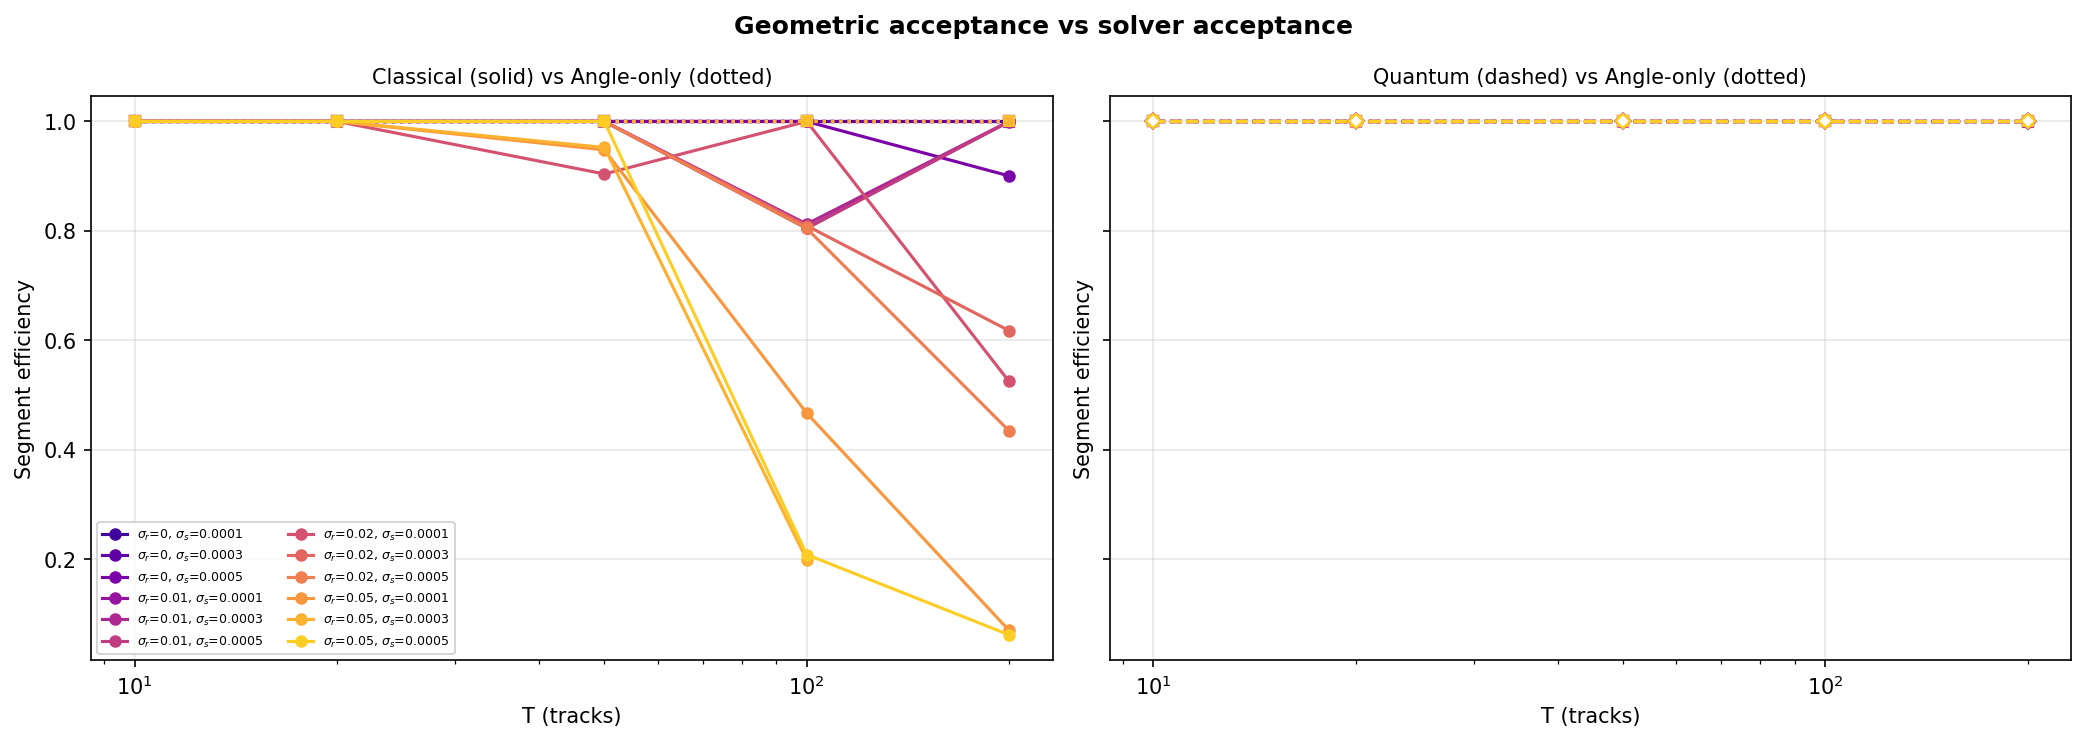
\includegraphics[width=\linewidth]
    {figures/deep_analysis/F_geometric_vs_solver/efficiency_comparison.png}
  \caption{Angle efficiency (geometric; dotted), classical efficiency (solid), and
    quantum efficiency corrected (dashed) vs $\ntrk$ for all 12 noise conditions.}
  \label{fig:geom_vs_solver}
\end{figure}

The angle-based acceptance is $\eta_\alpha=1.000$ throughout, confirming that $\eps$
correctly passes all true triplets in all conditions (Fig.~\ref{fig:geom_vs_solver}).
Classical efficiency collapses below $\eta_\alpha$ at high $\ntrk$ and noise; quantum
efficiency tracks $\eta_\alpha=1.000$ across the entire landscape.  The efficiency
failure is therefore entirely in the linear-system solver, not in the geometric filter.

\subsection{Timing and Quantum Resource Scaling}
\label{sec:results:timing}

\begin{figure}[H]
  \centering
  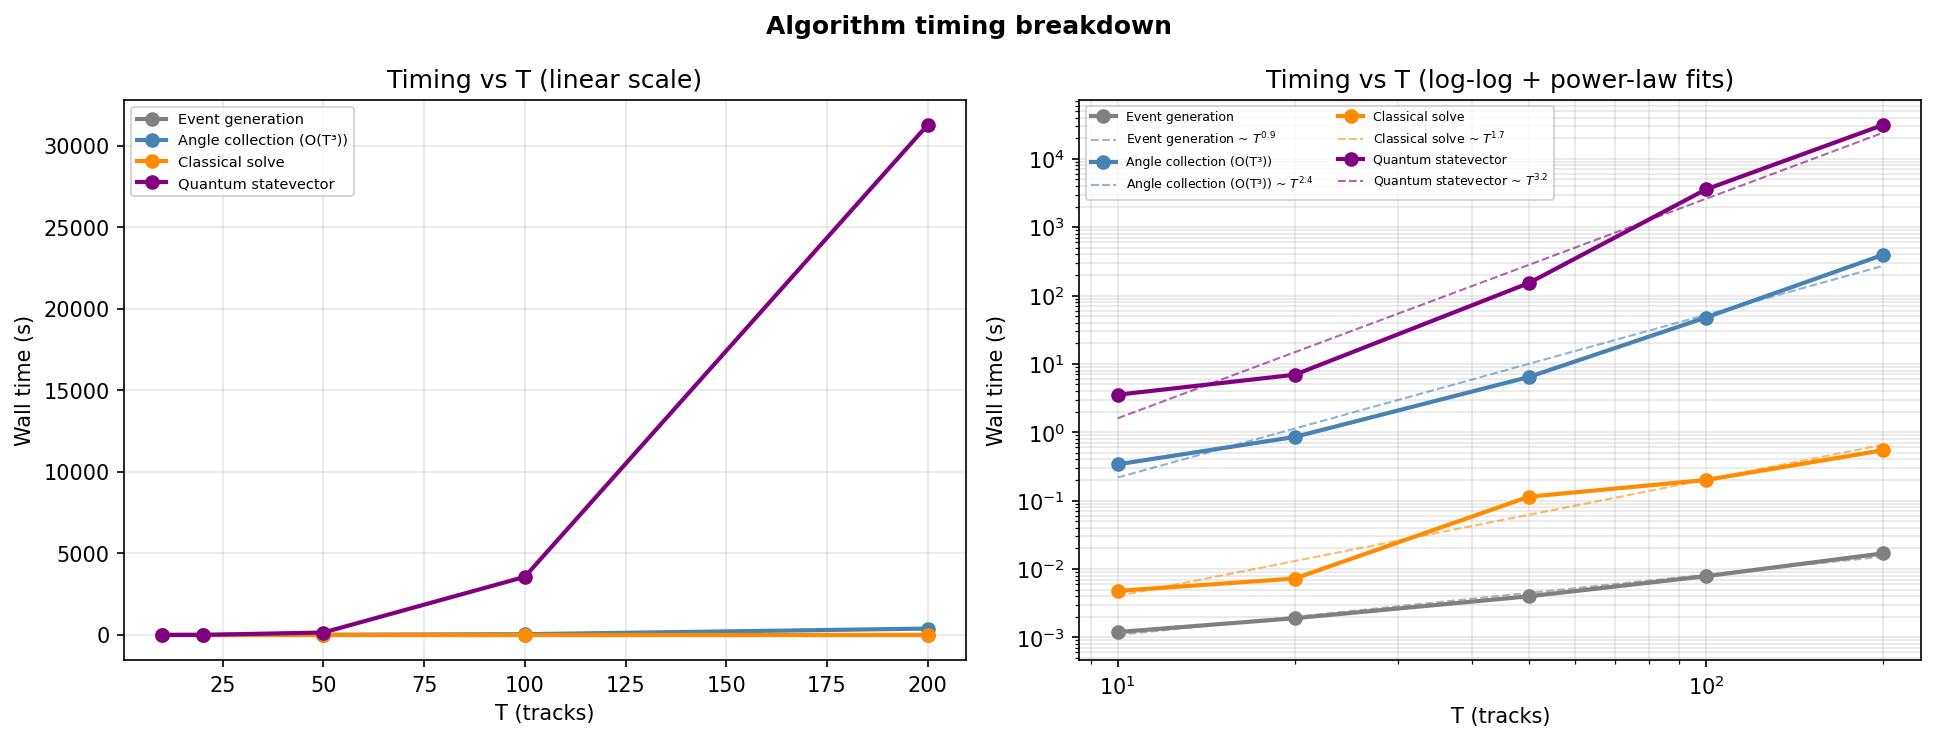
\includegraphics[width=0.80\linewidth]
    {figures/deep_analysis/G_timing/timing_vs_T.png}
  \caption{Wall-clock solve times vs $\ntrk$ on log--log scale with power-law fits.
    Dashed coloured lines show the fits.}
  \label{fig:timing}
\end{figure}

Power-law fits from Fig.~\ref{fig:timing} give:
\begin{align}
  t_{\rm classical} &\sim \ntrk^{1.9} \quad (\text{sparse direct/CG solve}),\\
  t_{\rm quantum}   &\sim \ntrk^{4.5} \quad (\text{classical statevector simulation}).
\end{align}
The quantum exponent reflects $t_q\propto 2^{n_{\rm qubits}}\propto\Nseg\propto\ntrk^2$.
A physical quantum device would execute the circuit in $O(\mathrm{poly}(n_{\rm qubits}))$
time, eliminating the exponential overhead.

\subsection{Full Landscape: Metrics vs Track Density and Noise}
\label{sec:results:landscape}

\begin{figure}[H]
  \centering
  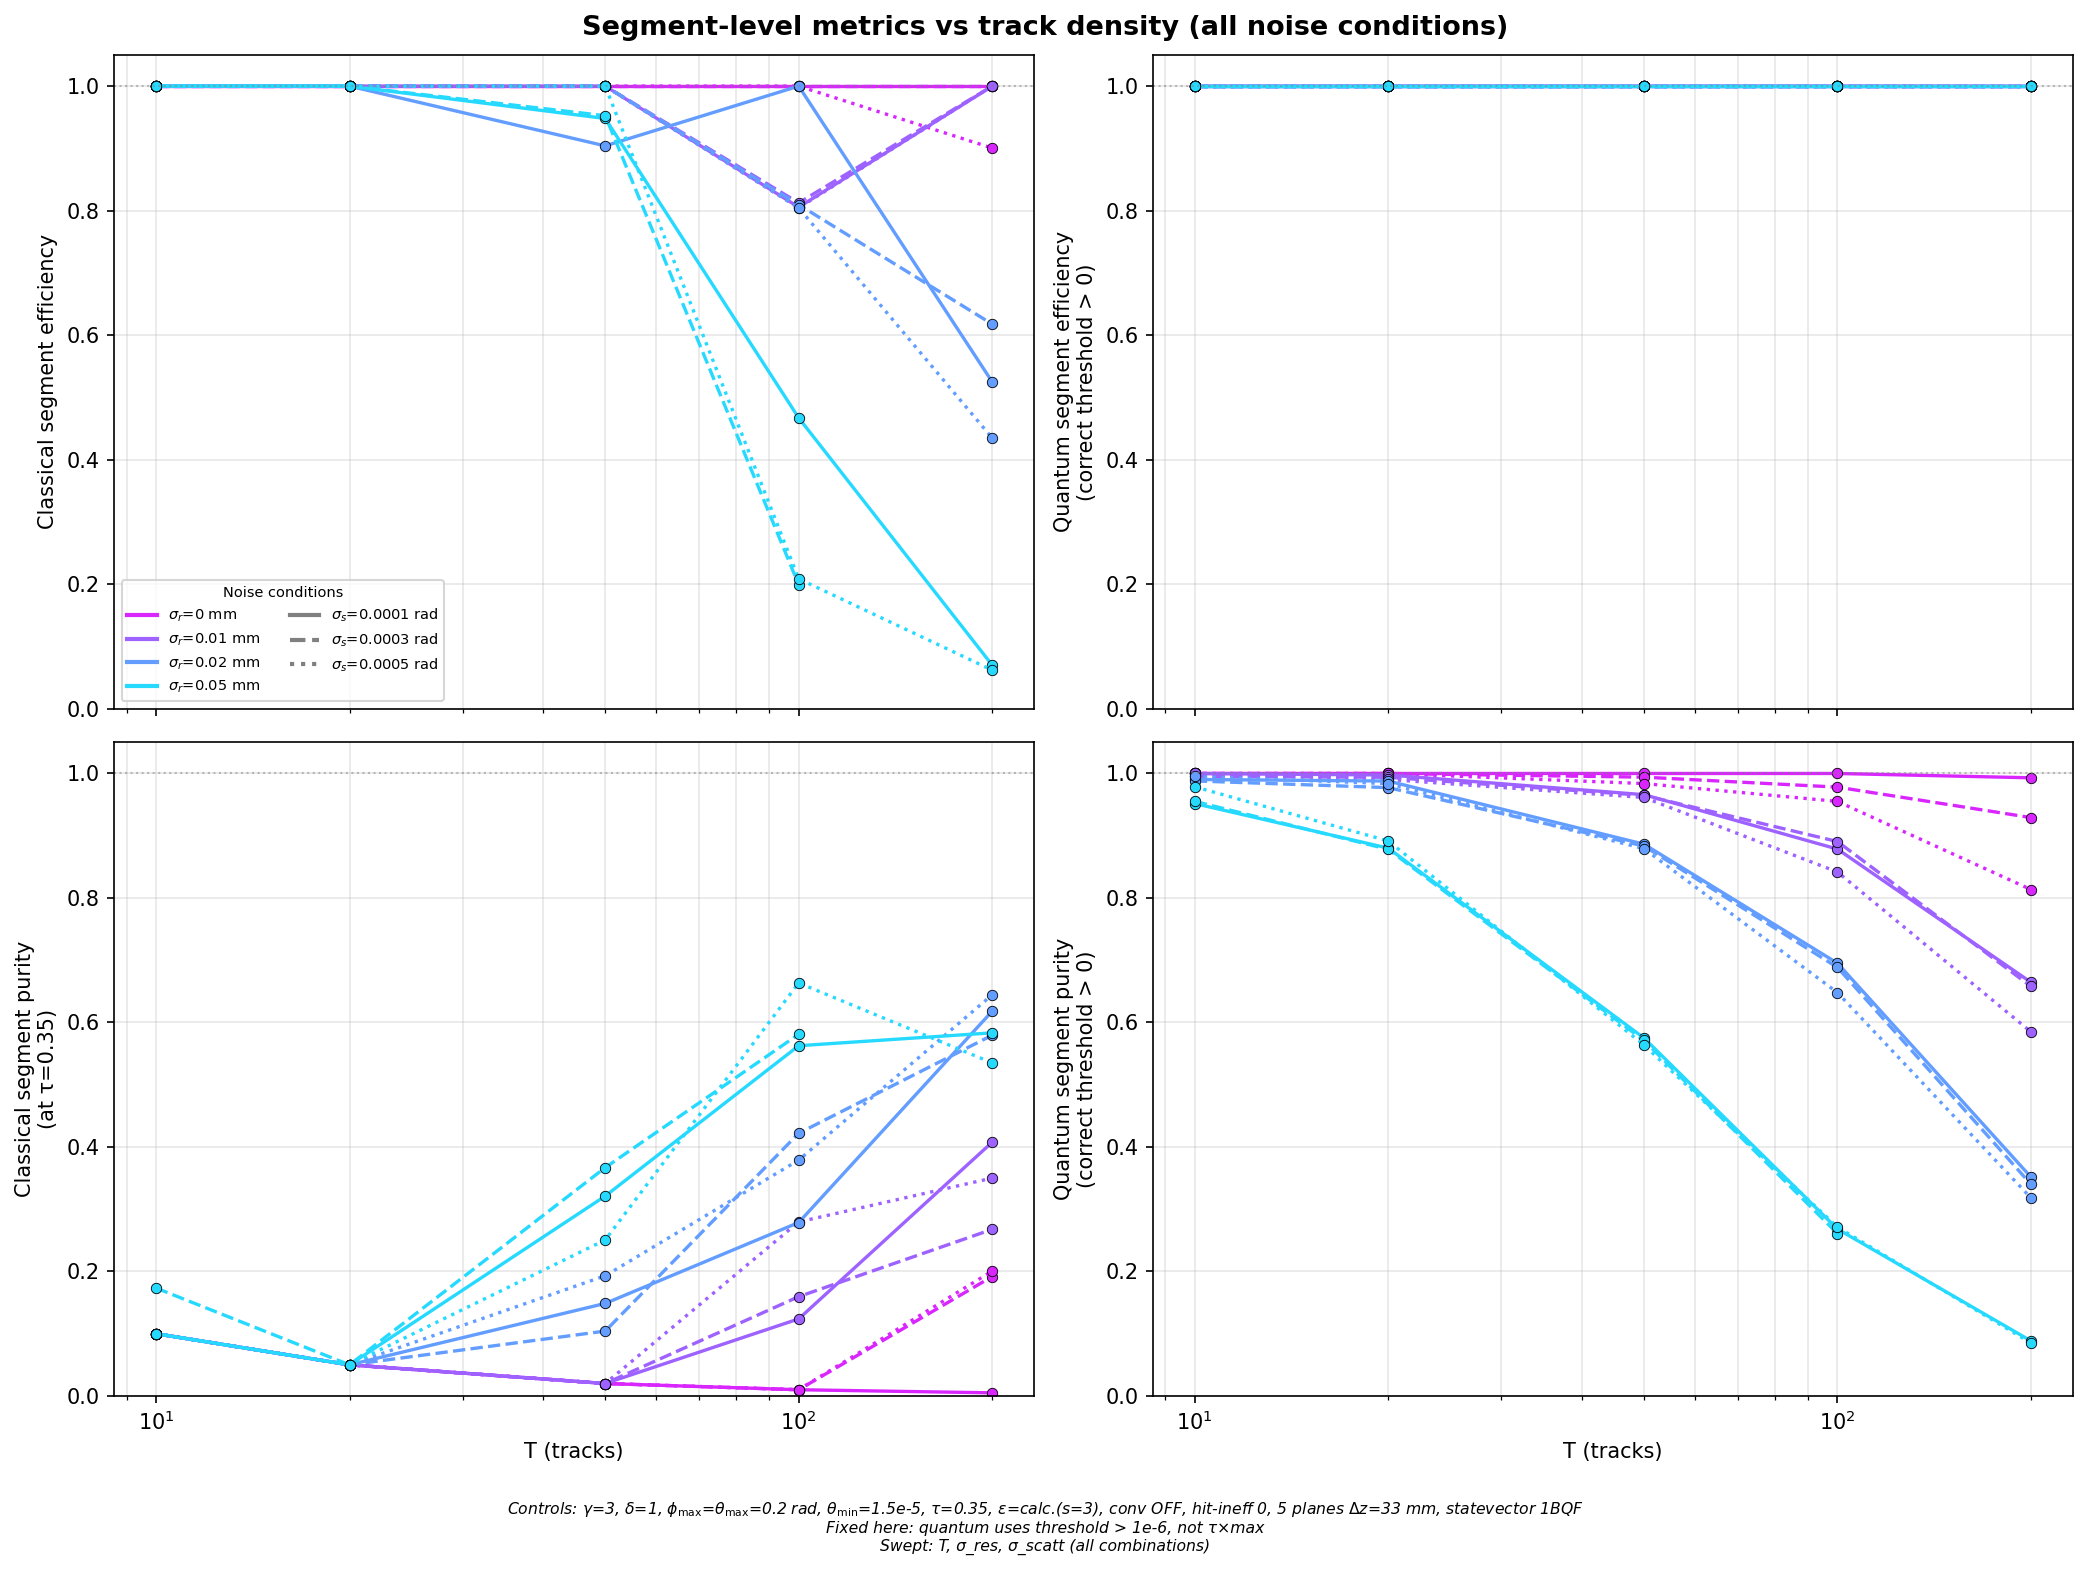
\includegraphics[width=\linewidth]
    {figures/deep_analysis/H_landscape/metrics_vs_T.png}
  \caption{The four key segment-level metrics vs $\ntrk$ for all 12 noise conditions.
    Line colour encodes $\sres$ (dark to light = low to high); linestyle encodes
    $\sscat$ (solid/dashed/dotted = low/mid/high).}
  \label{fig:metrics_vs_T}
\end{figure}

\begin{figure}[H]
  \centering
  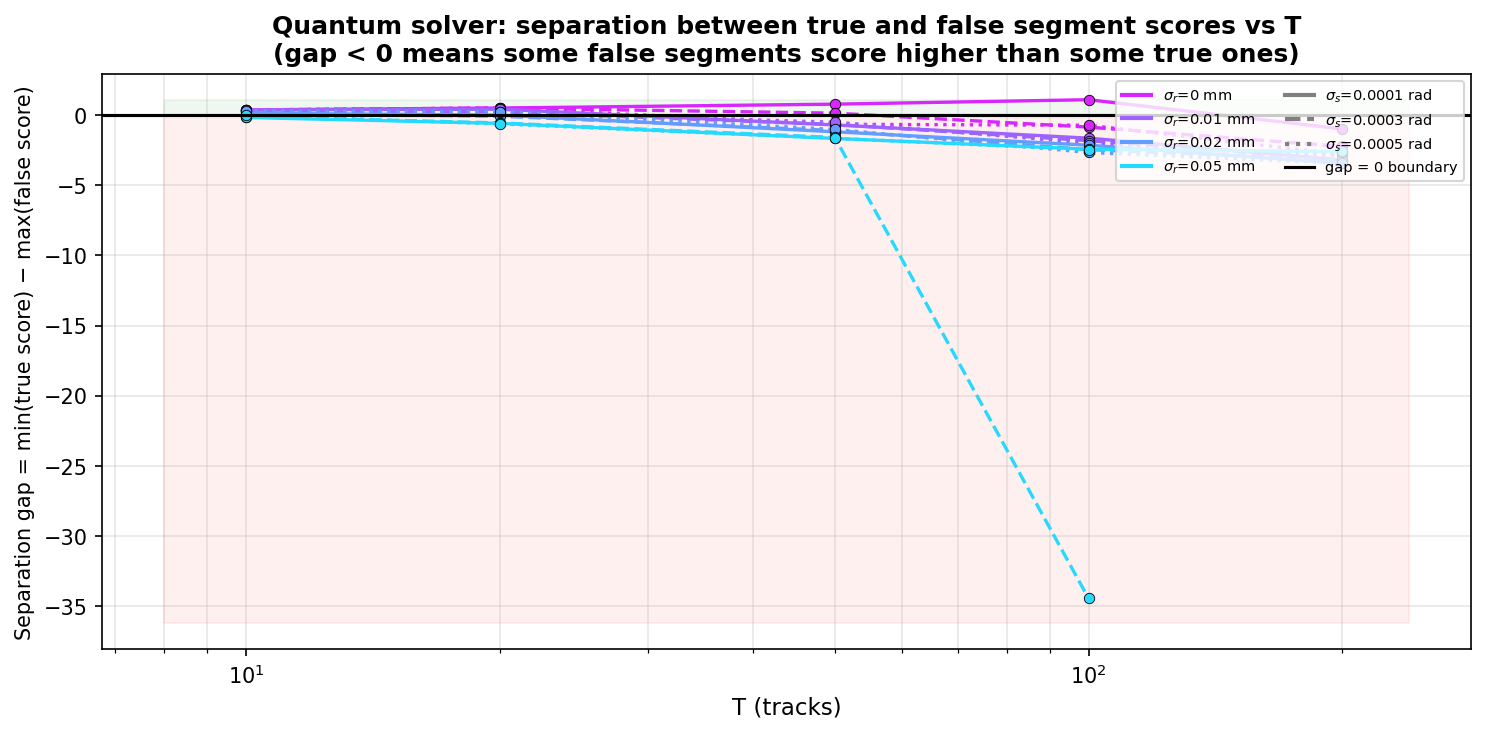
\includegraphics[width=\linewidth]
    {figures/deep_analysis/H_landscape/quantum_gap_vs_T.png}
  \caption{Quantum separation gap $\Delta_Q$ vs $\ntrk$ for all noise conditions.
    The black horizontal line is the false-leakage boundary $\Delta_Q=0$.
    Green shading indicates perfect separation; red shading the leakage regime.}
  \label{fig:gap_vs_T}
\end{figure}

\begin{figure}[H]
  \centering
  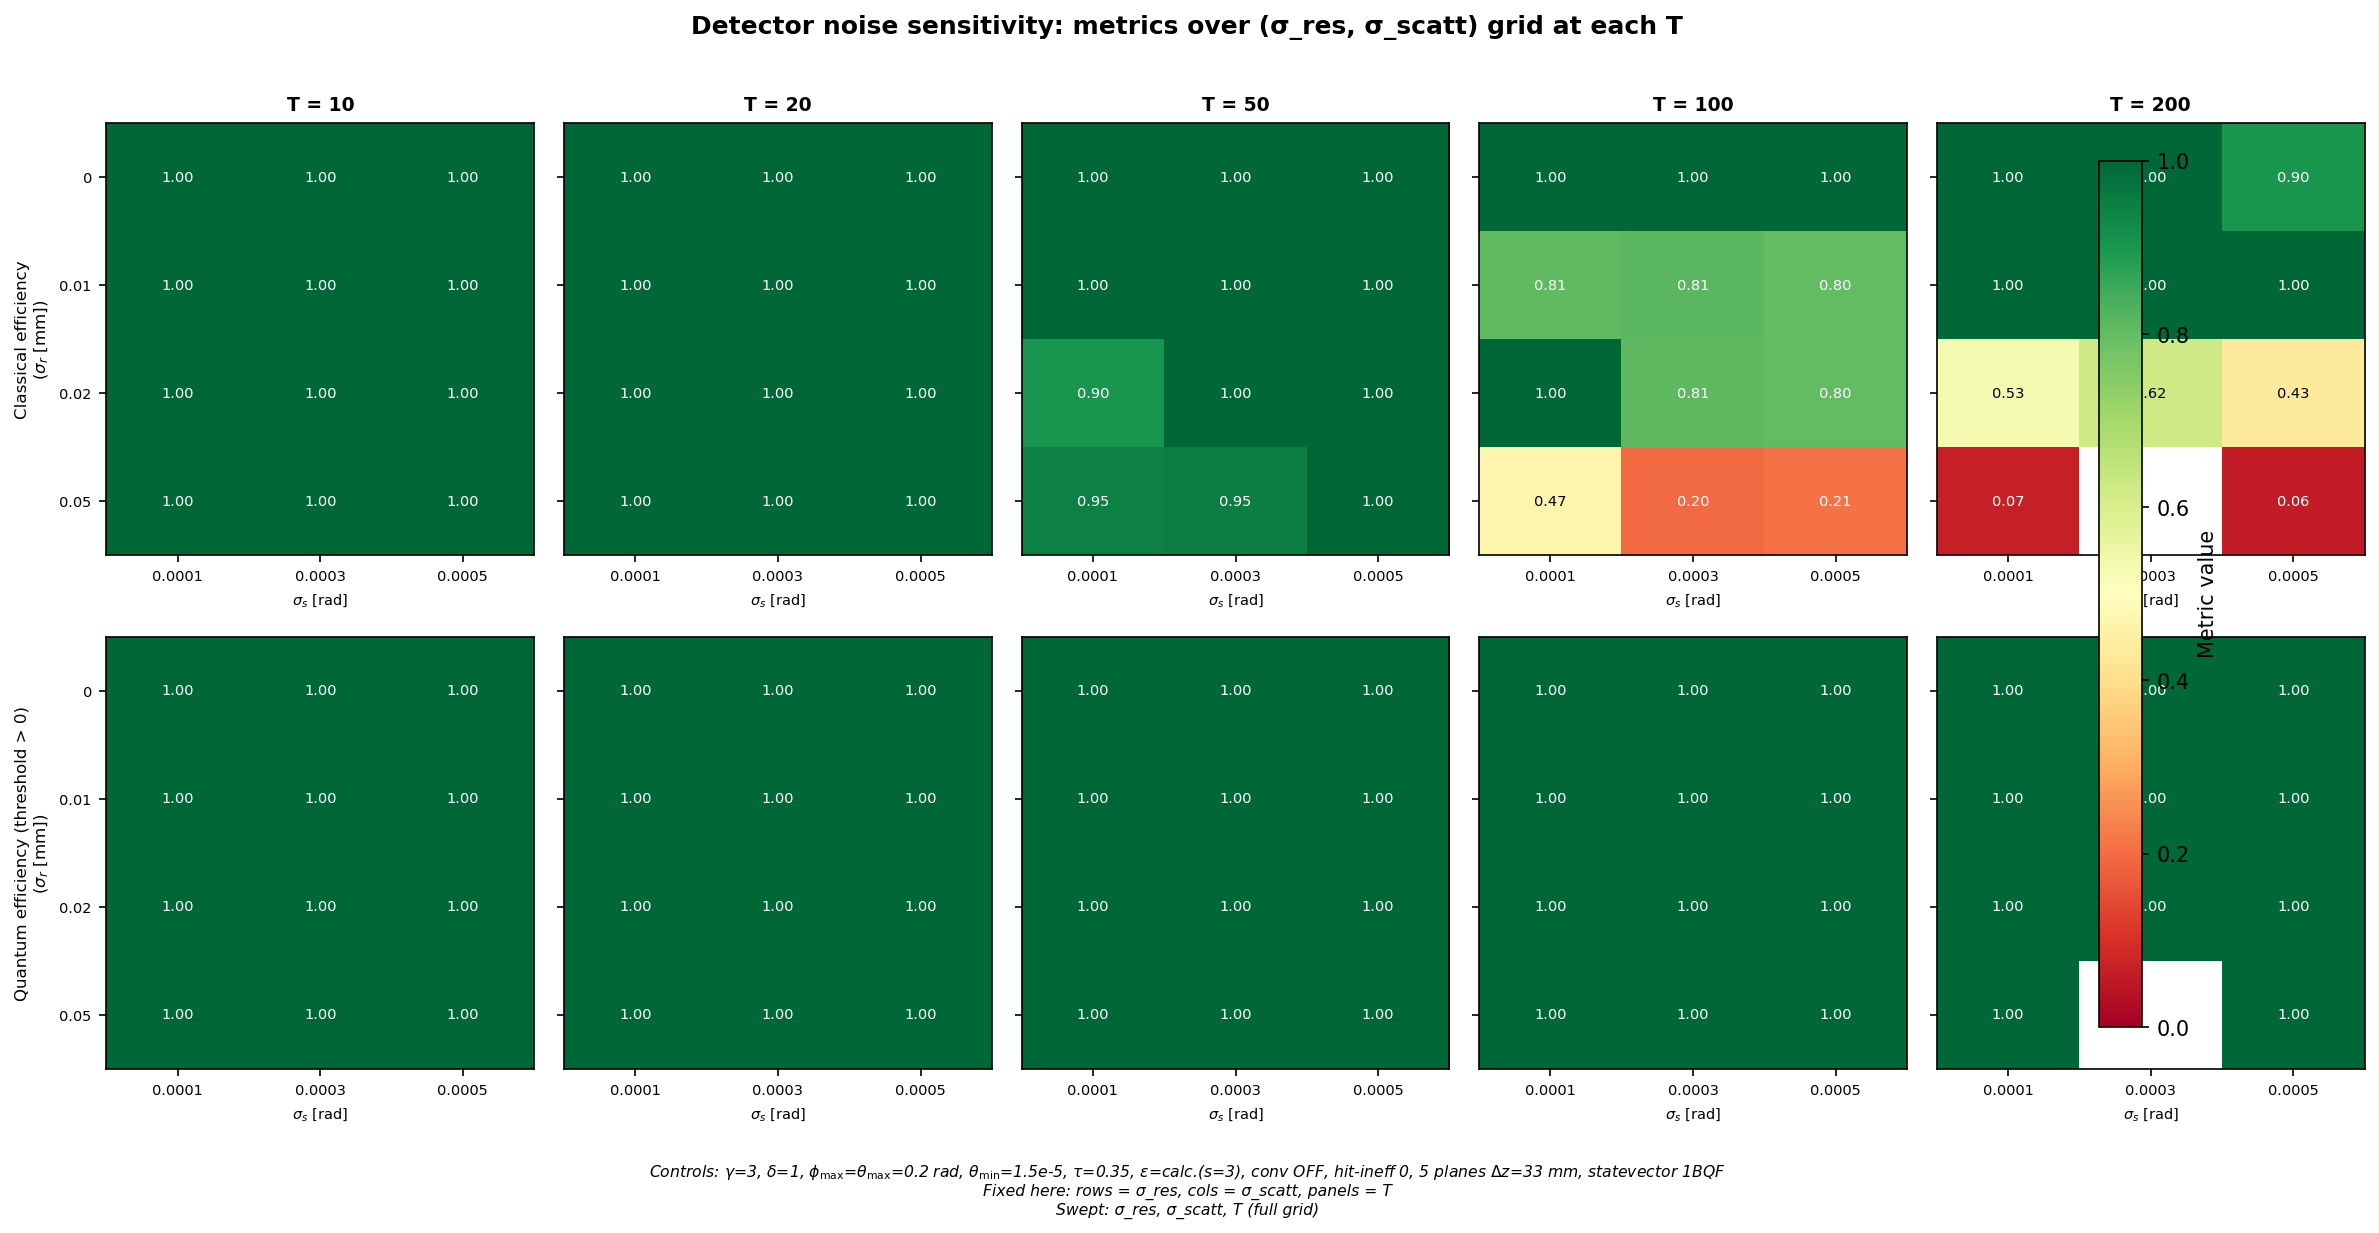
\includegraphics[width=\linewidth]
    {figures/deep_analysis/H_landscape/heatmap_efficiency.png}
  \caption{Classical (top row) and quantum (bottom row) segment efficiency over the
    $4\times3$ noise grid at each $\ntrk$.}
  \label{fig:heatmap_eff}
\end{figure}

\begin{figure}[H]
  \centering
  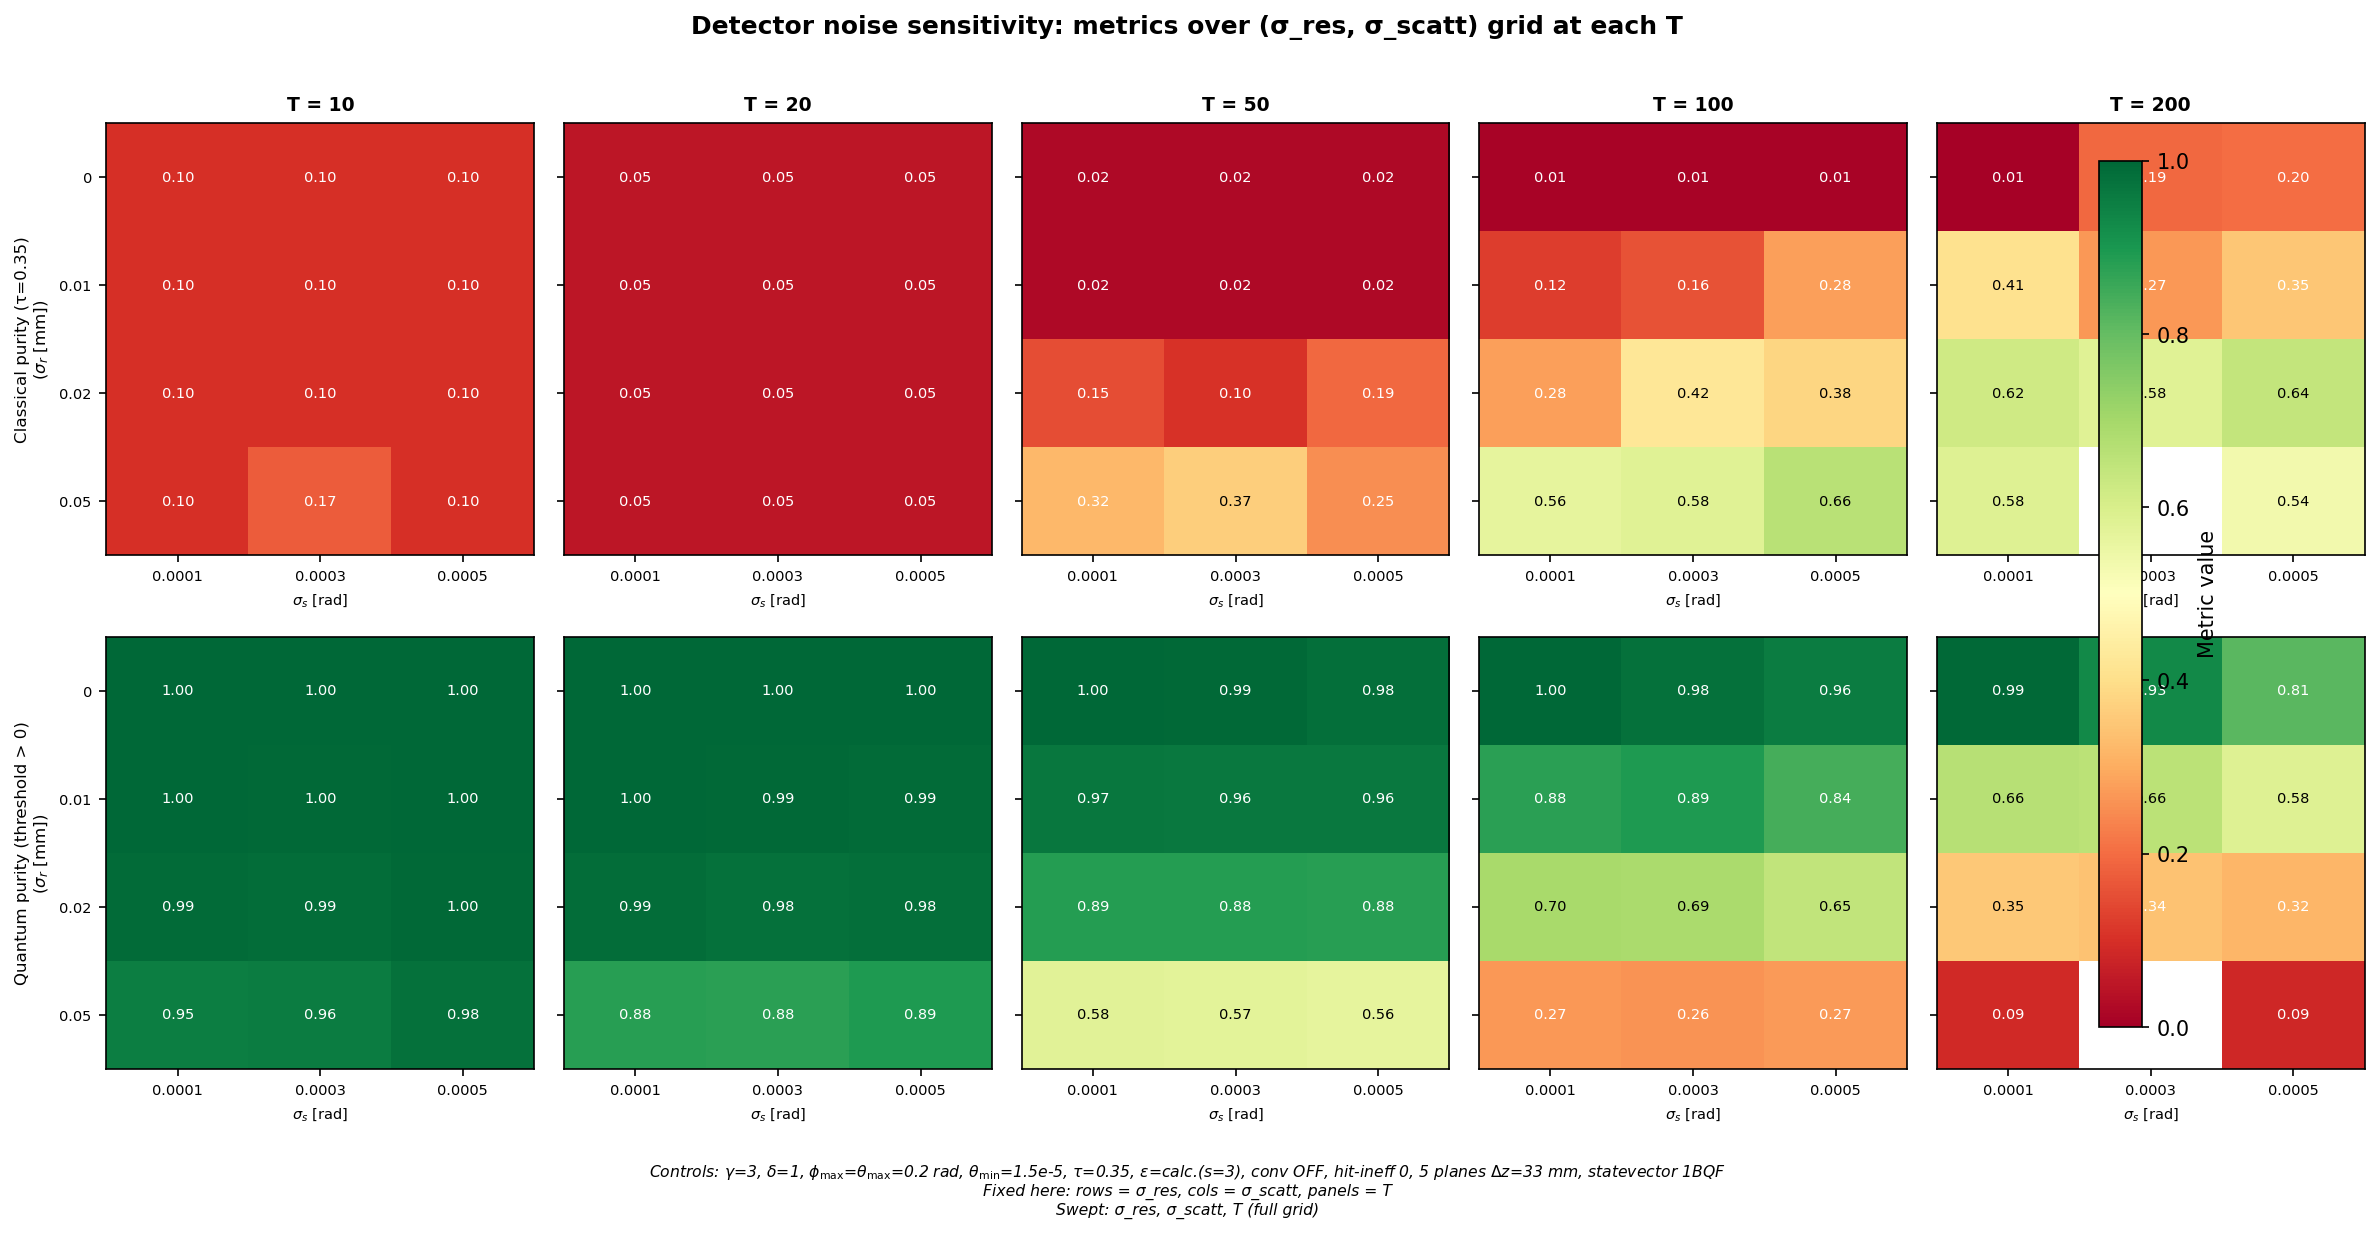
\includegraphics[width=\linewidth]
    {figures/deep_analysis/H_landscape/heatmap_purity.png}
  \caption{Classical (top row) and quantum (bottom row) segment purity over the
    $4\times3$ noise grid at each $\ntrk$.}
  \label{fig:heatmap_pur}
\end{figure}

Figures~\ref{fig:metrics_vs_T}--\ref{fig:heatmap_pur} reveal the full landscape:

\begin{itemize}
  \item \textbf{Classical efficiency} (Fig.~\ref{fig:heatmap_eff}, top) degrades
        primarily along the $\sres$ axis.  Collapse begins at $\ntrk=50$ for
        $\sres=0.05\,\mathrm{mm}$; the minimum at $\ntrk=200$ is $6\,\%$.
  \item \textbf{Quantum efficiency} (Fig.~\ref{fig:heatmap_eff}, bottom) is
        $1.000$ throughout.
  \item \textbf{Classical purity} (Fig.~\ref{fig:heatmap_pur}, top) appears to
        improve at high $\ntrk$ and noise --- an artefact of the solver missing
        most true segments while still activating some false ones.
  \item \textbf{Quantum purity} (Fig.~\ref{fig:heatmap_pur}, bottom) degrades
        smoothly.  $\sres$ dominates; at $\ntrk=200$, $\sres=0.05\,\mathrm{mm}$,
        purity falls to $\approx\!9\,\%$.
\end{itemize}

\subsection{Score Distribution Evolution with Track Density}
\label{sec:results:score_evo}

\begin{figure}[H]
  \centering
  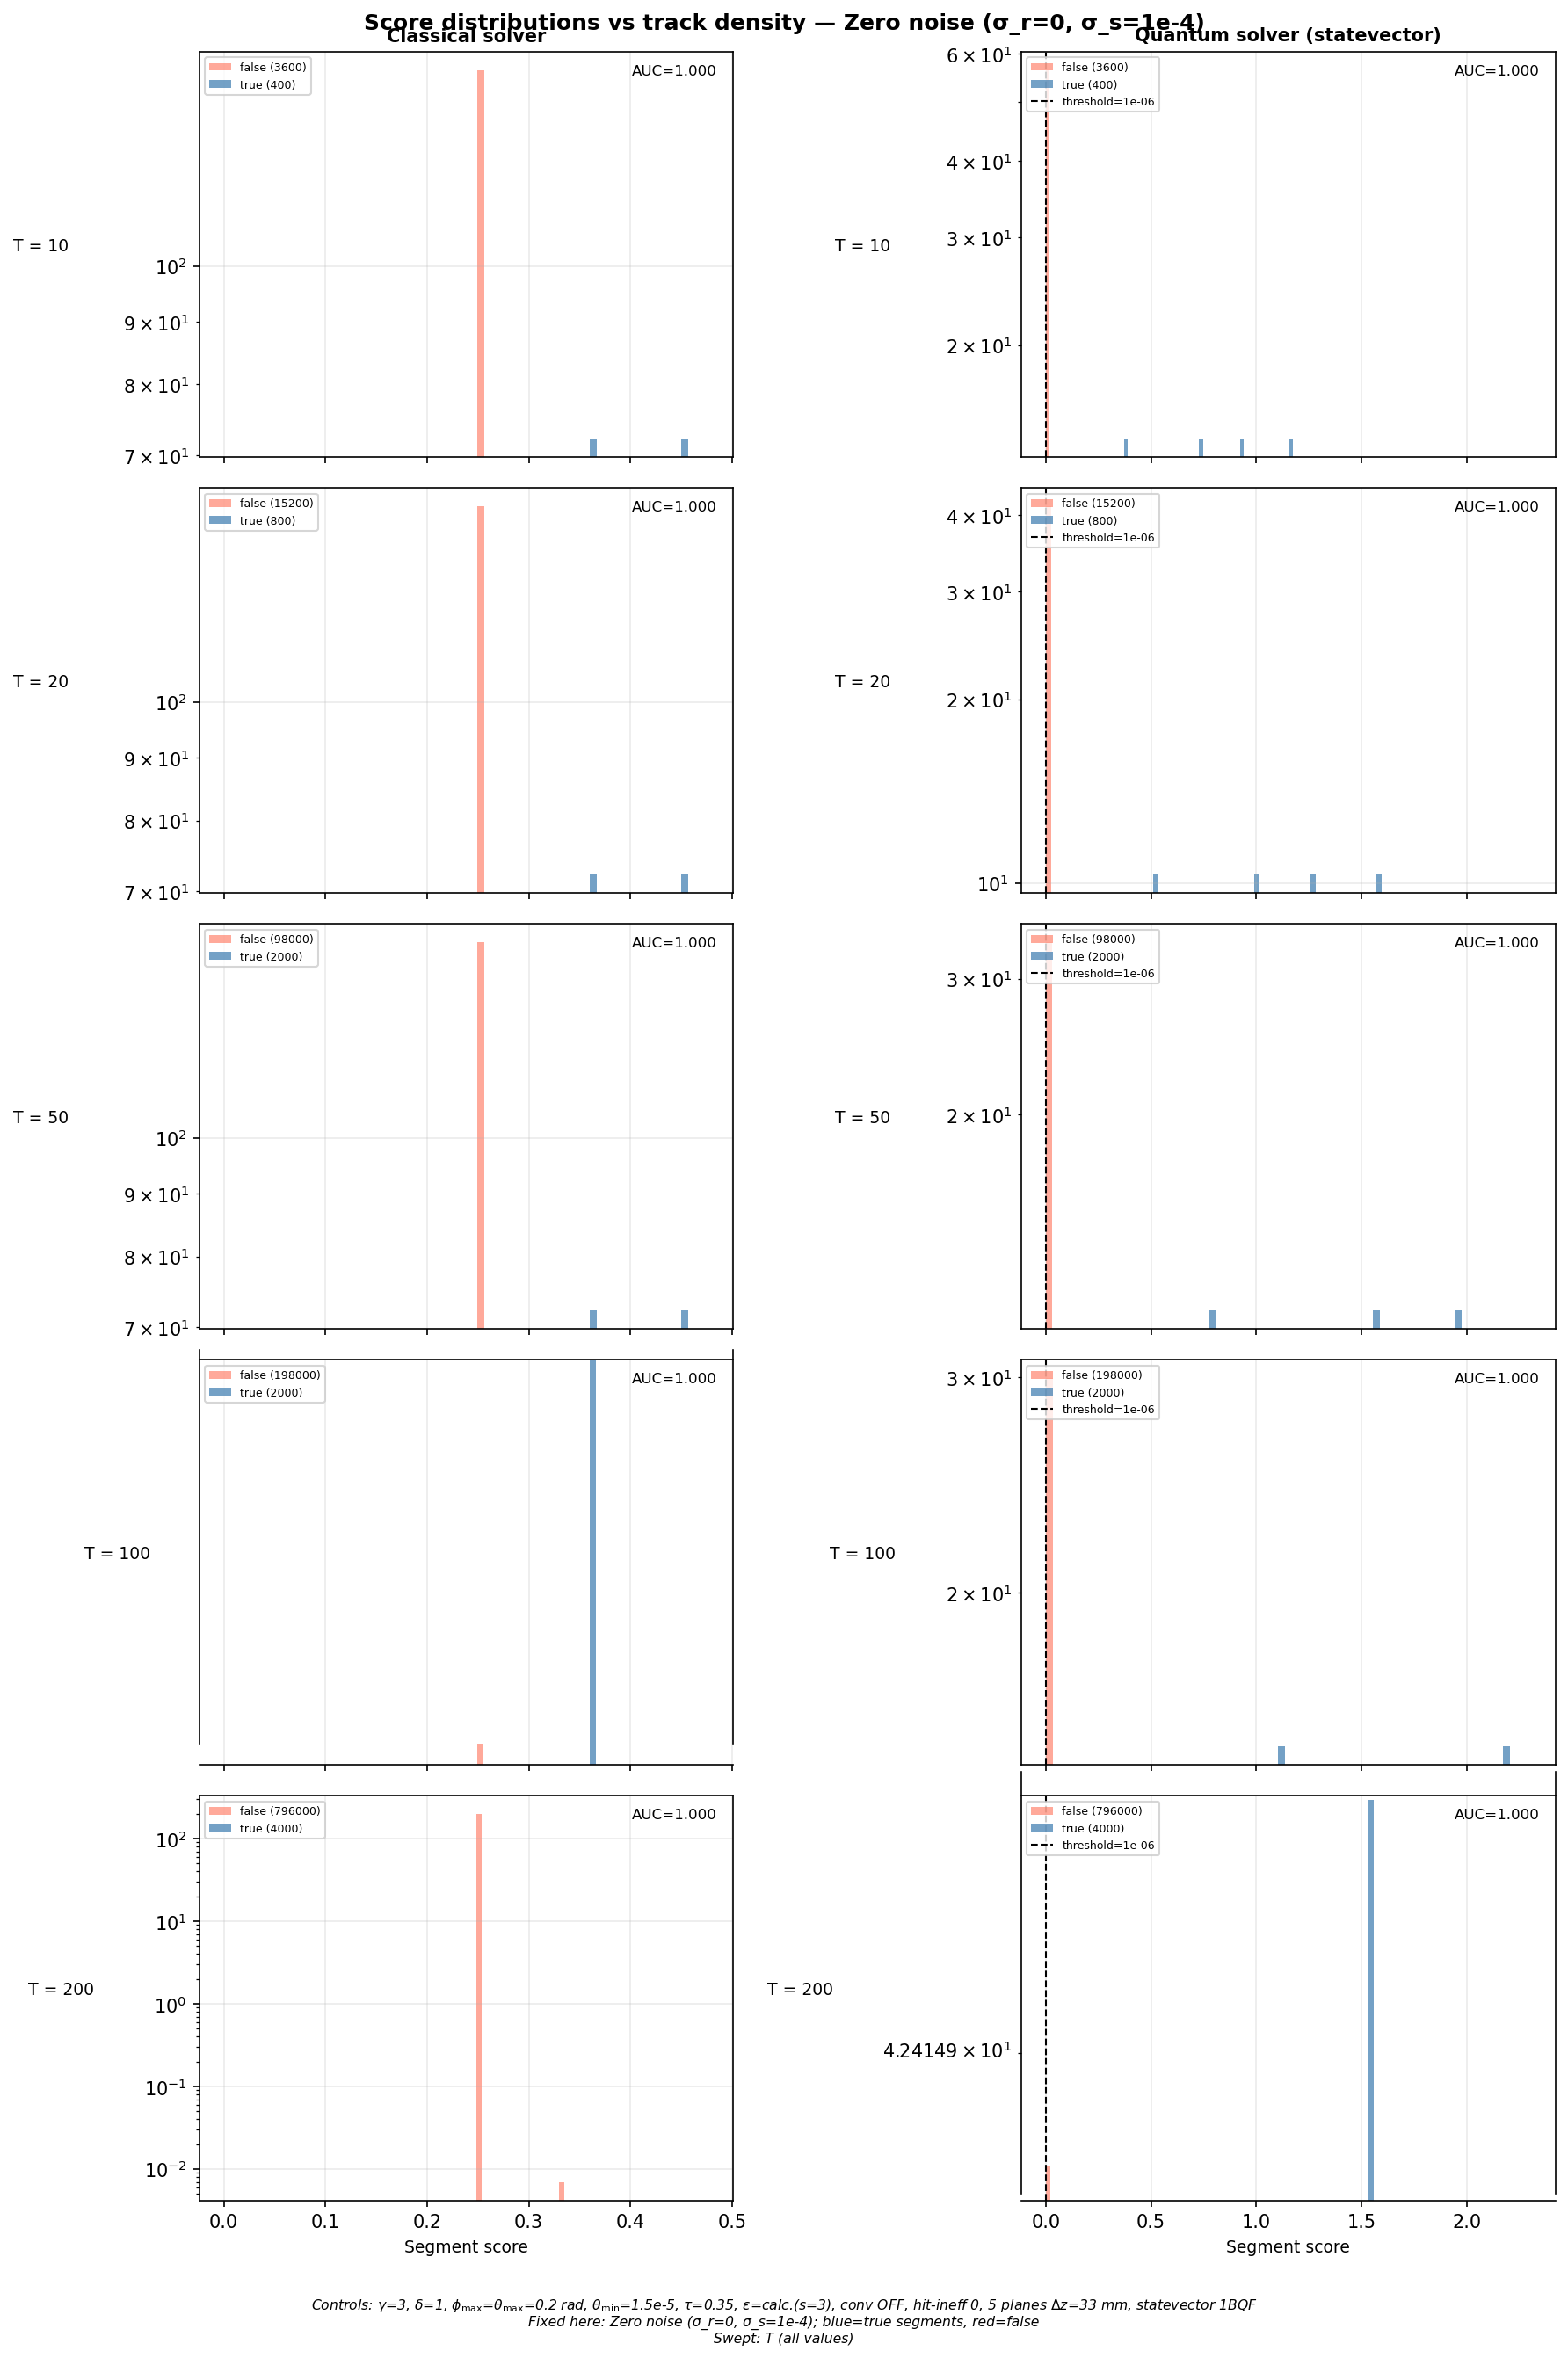
\includegraphics[width=\linewidth]
    {figures/deep_analysis/I_score_evolution/score_evolution_best.png}
  \caption{Classical and quantum score distributions at
    $\ntrk=10, 20, 50, 100, 200$ for zero noise
    ($\sres=0$, $\sscat=10^{-4}$~rad).
    Blue = true segments, red = false.  Log-scale density.}
  \label{fig:score_evo_best}
\end{figure}

\begin{figure}[H]
  \centering
  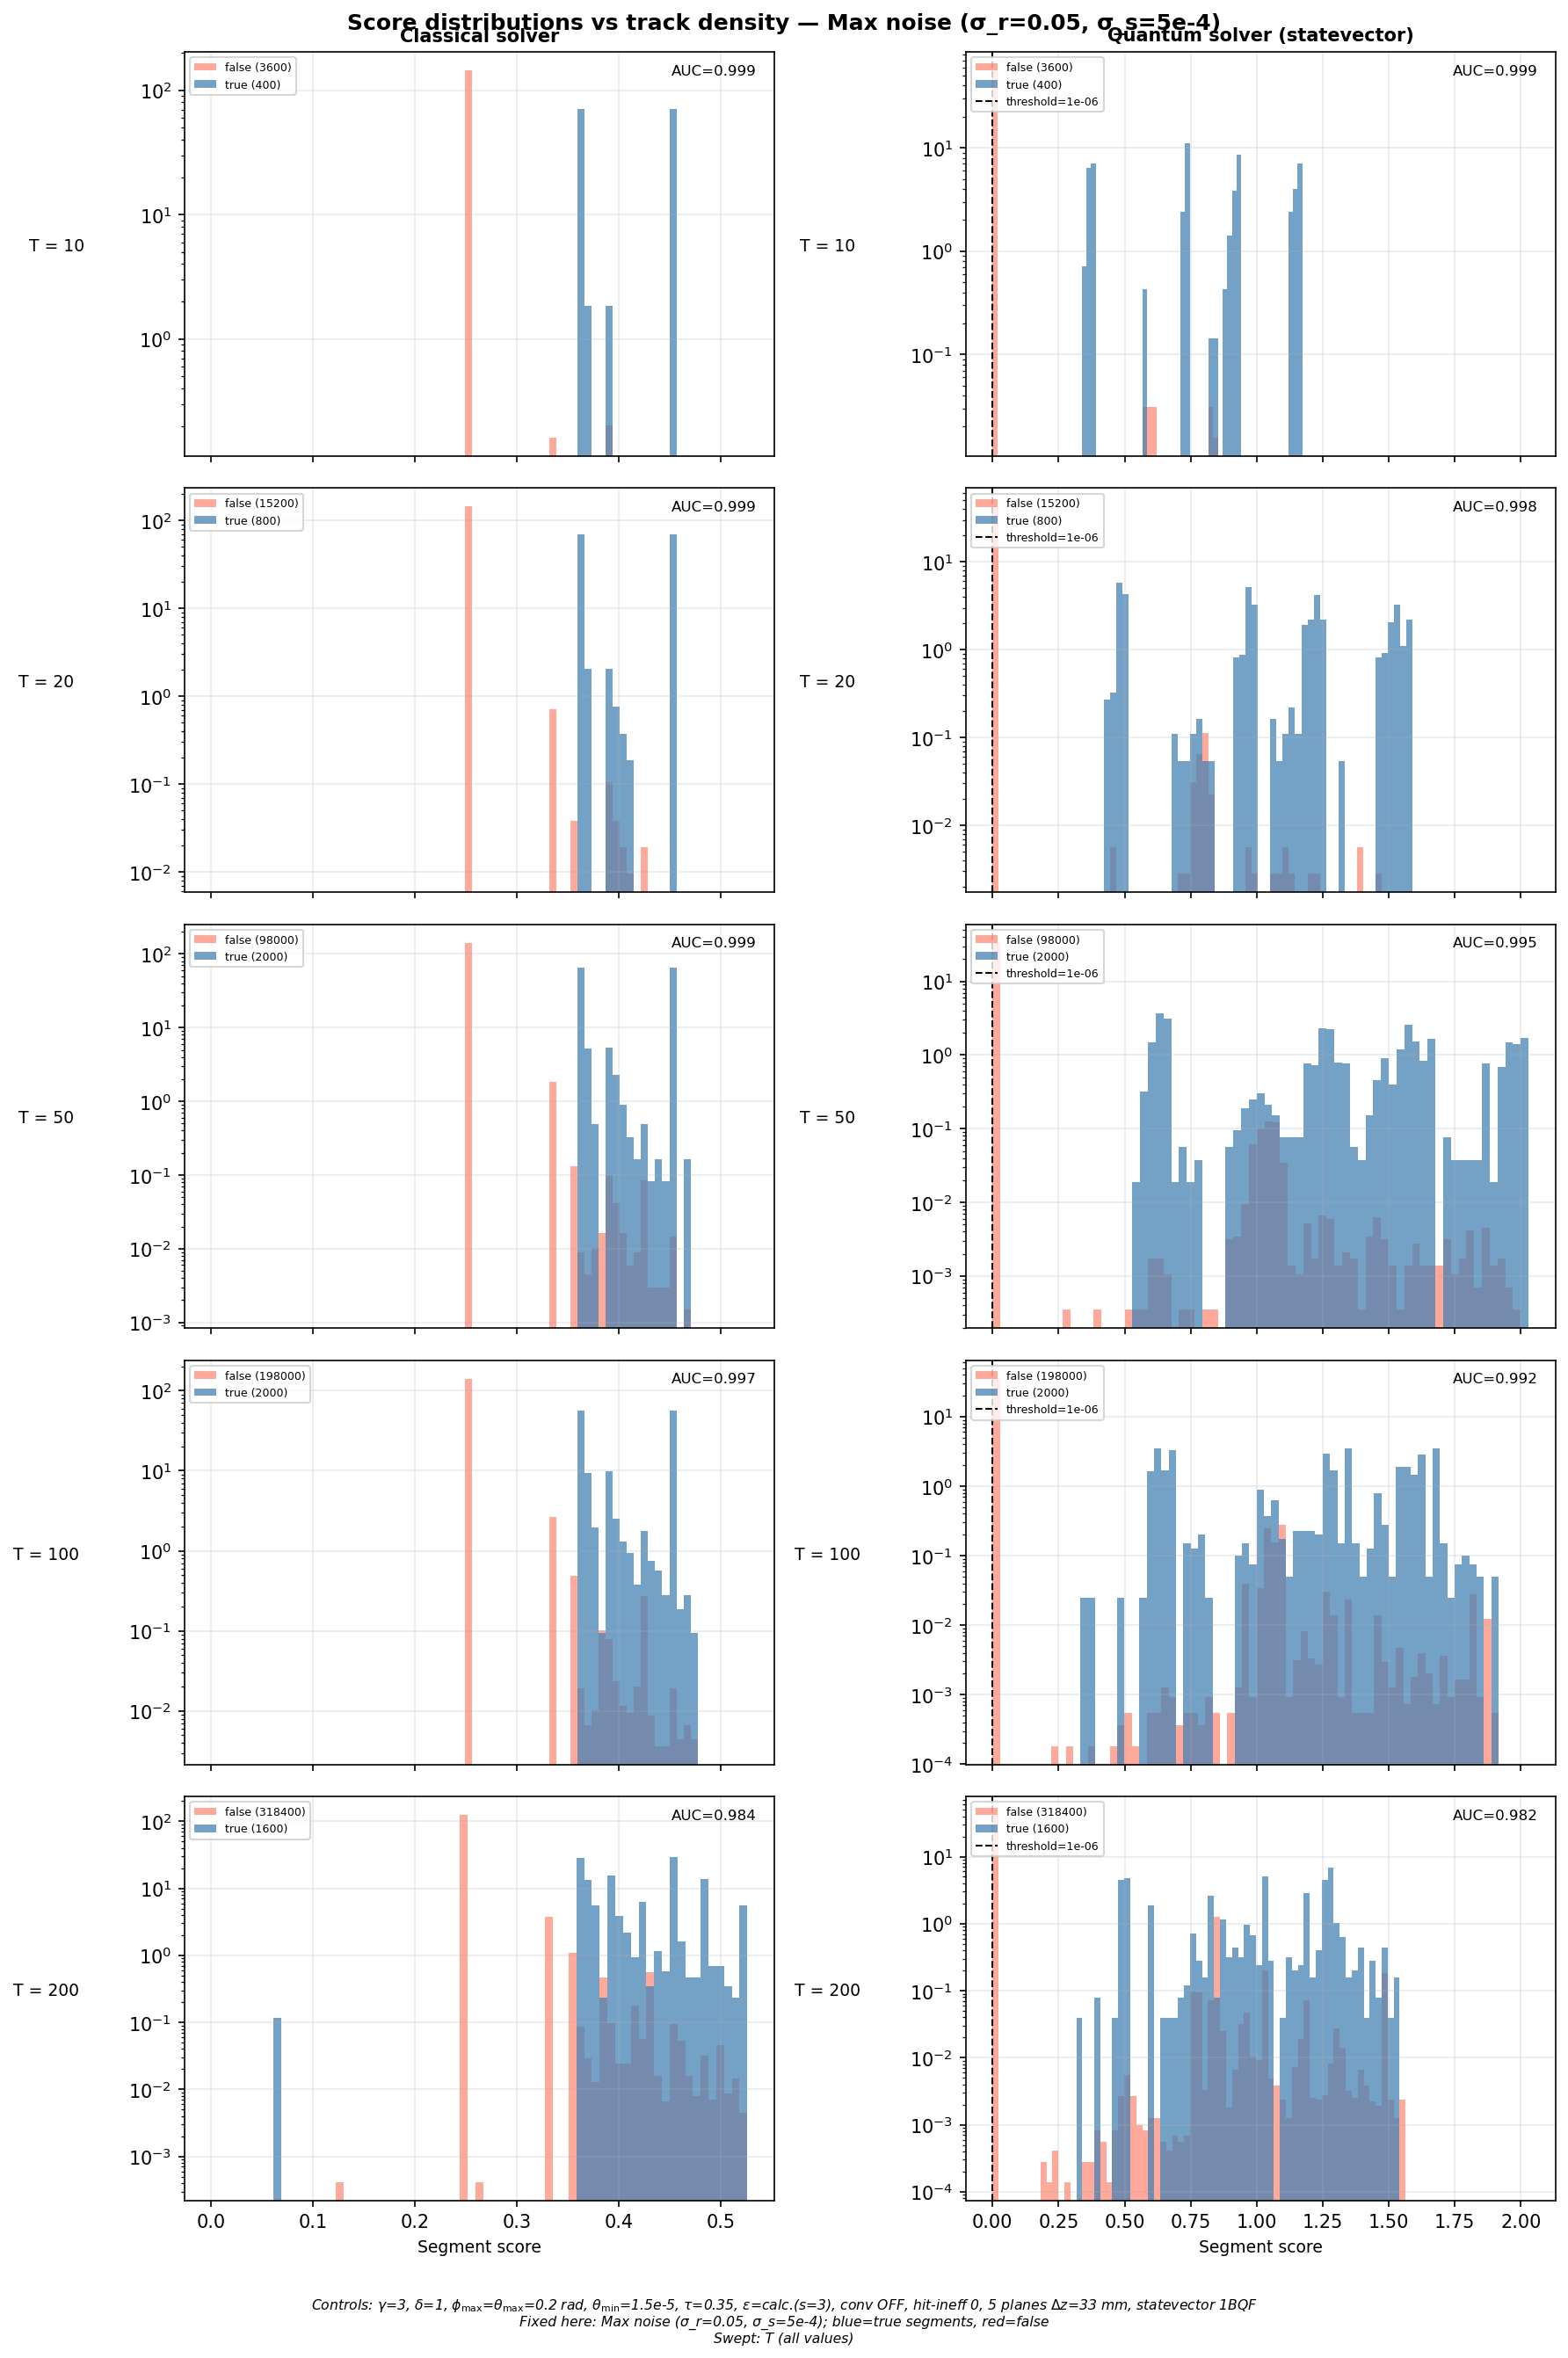
\includegraphics[width=\linewidth]
    {figures/deep_analysis/I_score_evolution/score_evolution_worst.png}
  \caption{As Fig.~\ref{fig:score_evo_best} but for maximum noise
    ($\sres=0.05\,\mathrm{mm}$, $\sscat=5\!\times\!10^{-4}$~rad).}
  \label{fig:score_evo_worst}
\end{figure}

\begin{figure}[H]
  \centering
  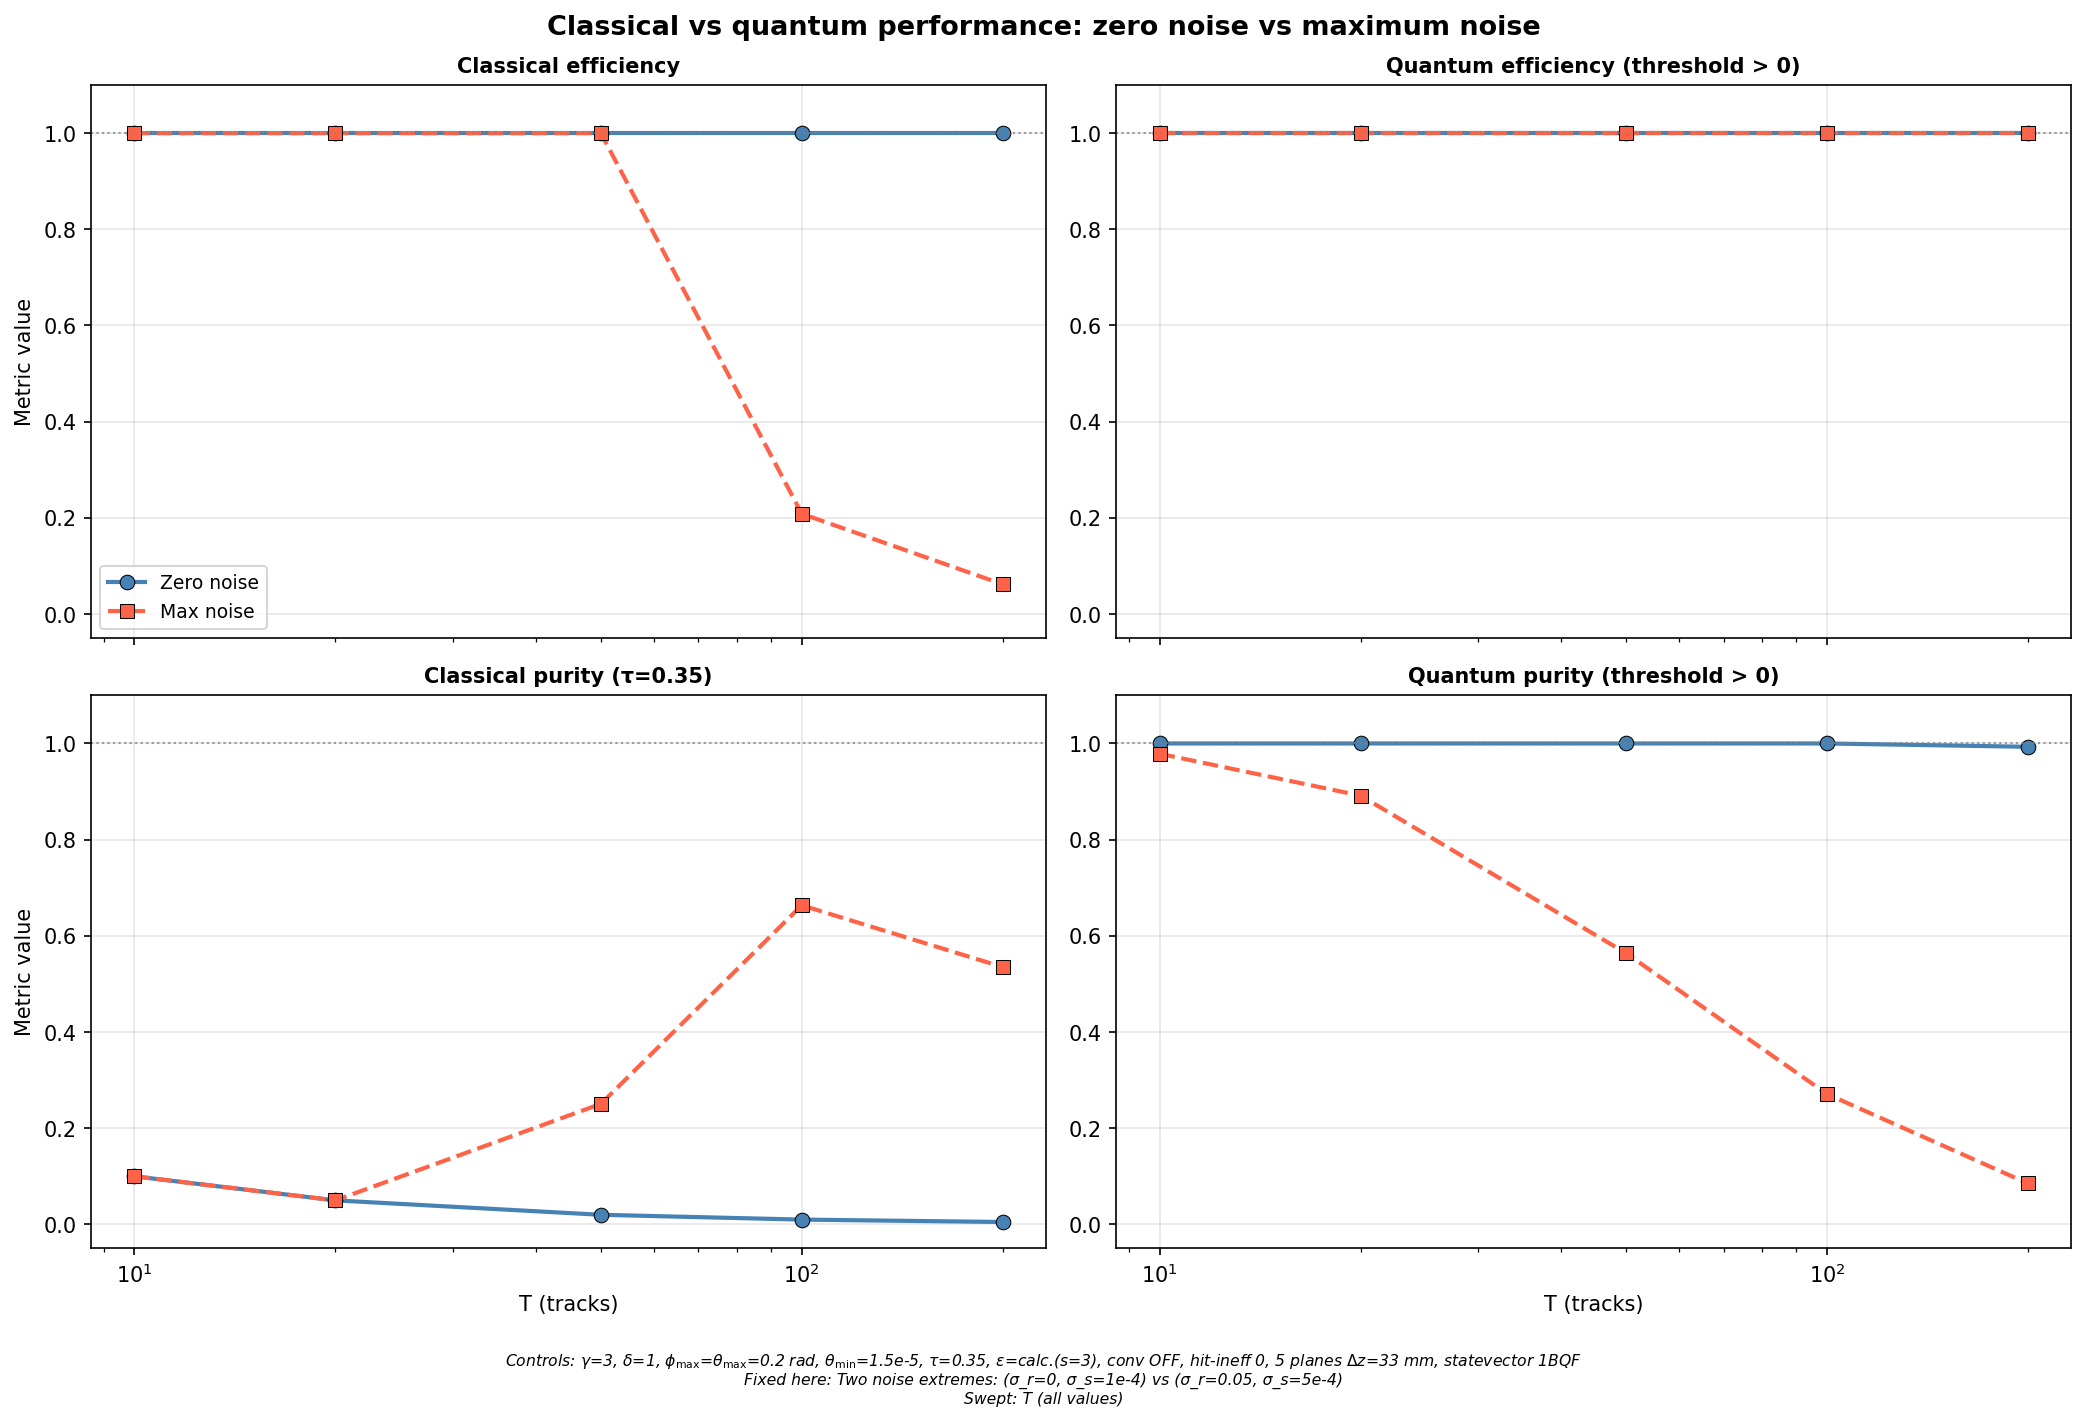
\includegraphics[width=\linewidth]
    {figures/deep_analysis/I_score_evolution/classical_vs_quantum_noise_comparison.png}
  \caption{All four metrics vs $\ntrk$ at the two noise extremes.  Blue circles:
    zero noise; red squares: maximum noise.}
  \label{fig:noise_comparison}
\end{figure}

At zero noise (Fig.~\ref{fig:score_evo_best}), classical score distributions remain
cleanly separated at all densities; quantum false scores stay at machine precision until
$\ntrk=200$.  At maximum noise (Fig.~\ref{fig:score_evo_worst}), classical
distributions merge completely from $\ntrk=50$ and the solver becomes effectively
random.  Fig.~\ref{fig:noise_comparison} presents the starkest summary: classical
efficiency collapses under maximum noise while quantum efficiency is invariant; the
``improved'' classical purity at maximum noise is an artefact of total efficiency
collapse.

% ══════════════════════════════════════════════════════════════════════════════
\subsection{Algorithm Stability: The Operating Envelope}
\label{sec:results:stability}

Consolidating Sections~\ref{sec:results:landscape}--\ref{sec:results:score_evo}, the
behaviour of the segment-level algorithm under detector noise separates into three
regimes, controlled almost entirely by the measurement resolution~$\sres$; the
multiple-scattering term~$\sscat$ is sub-dominant over the range studied.
Table~\ref{tab:stability} summarises this operating envelope.

\begin{table}[H]
  \centering
  \caption{Operating envelope of the segment-level algorithm. The measurement
    resolution $\sres$ is the controlling axis; $\sscat$ shifts the boundaries only
    weakly. Efficiency/purity values are segment-level, at the validated operating
    point ($\tau=0.35$ classical, absolute threshold $x_Q>\Qthresh$ quantum).}
  \label{tab:stability}
  \small
  \begin{tabular}{p{1.7cm}p{4.2cm}p{7.2cm}}
    \toprule
    Regime & Condition & Solver behaviour \\
    \midrule
    \textbf{Stable} & $\sres\leq0.01\,\mathrm{mm}$, all $\ntrk$ tested &
      Classical \emph{and} quantum efficiency $=1.00$; true/false scores remain
      bimodally separated; reproduces the Verify\_new\_results benchmark. \\[2pt]
    \textbf{Marginal} & $\sres=0.02\,\mathrm{mm}$, $\ntrk\gtrsim50$ &
      Classical efficiency begins to fall; quantum efficiency still $1.00$ but
      purity starts to drop as the separation gap $\Delta_Q$ approaches zero. \\[2pt]
    \textbf{Broken} & $\sres=0.05\,\mathrm{mm}$, $\ntrk\geq100$ &
      Classical efficiency collapses to $0.06$ at $\ntrk=200$ (cliff edge, no $\tau$
      recovers it); quantum efficiency $=1.00$, purity falls smoothly to $0.09$. \\
    \bottomrule
  \end{tabular}
\end{table}

Three points characterise the stability of the algorithm.

\begin{enumerate}[topsep=2pt]
  \item \textbf{Where the algorithm is stable.}
        For $\sres\leq0.01\,\mathrm{mm}$ both solvers reproduce the noise-free benchmark
        at every density tested ($\ntrk\leq200$): geometric (angle) efficiency, classical
        efficiency and quantum efficiency all sit at $1.00$ within statistics, matching
        the Verify\_new\_results baseline that defines the validated operating point.
        The segment scores stay cleanly bimodal (Fig.~\ref{fig:score_evo_best}), so the
        whole pipeline --- $\eps$ acceptance, Hamiltonian, both solvers --- is stable and
        density-independent in this regime.

  \item \textbf{Where noise overwhelms the segments.}
        The segment representation itself breaks down once
        $\sres\gtrsim0.02\,\mathrm{mm}$ \emph{and} $\ntrk\gtrsim50$. The true-triplet
        kink-angle spread then grows to the order of the inter-track angular separation,
        so genuine and accidental triplets become geometrically indistinguishable: the
        true and false score distributions merge (Fig.~\ref{fig:score_evo_worst}) while
        the false pool ($\propto\ntrk^2$) swamps the signal. Crucially this is a property
        of the \emph{segment data}, not of either solver --- the $\eps$ formula still
        accepts $\geq99.97\,\%$ of true triplets, but acceptance no longer implies
        discrimination. No downstream solver or threshold can recover information the
        segments no longer carry.

  \item \textbf{How each solver degrades --- the stability signature.}
        The two solvers fail in qualitatively different ways. The classical solver shows
        a \emph{cliff edge}: efficiency holds at $1.00$ until the dominant eigenvector of
        $A$ flips from the true- to the false-segment subspace, then collapses to $0.06$
        with no threshold able to recover it. The TrackHHL quantum solver is
        \emph{conditionally stable}: its efficiency is invariant at $1.00$ across the
        entire landscape, and degradation appears only as graceful purity loss
        (false-segment leakage), tracked by the gap $\Delta_Q$ crossing zero
        (Fig.~\ref{fig:gap_vs_T}). Within the envelope the algorithm is stable for both
        solvers; beyond it the classical solver loses the signal entirely, whereas the
        quantum solver retains every true segment and fails only by admitting false ones.
\end{enumerate}

% ══════════════════════════════════════════════════════════════════════════════
\section{Discussion}
\label{sec:discussion}

\subsection{The $\varepsilon$ Formula}

The formula achieves its design goal across the full noise range.  The
$\approx\!55\,\%$ overestimate of $\srkink$ reflects the worst-case quadrature
construction.  The overestimate is noise-independent and density-independent, pointing
to the analytic derivation rather than a data artefact.  A tighter formula or a
per-event adaptive $\eps$ could reduce false-segment coupling by $\approx\!30\,\%$
without sacrificing coverage.

\subsection{Classical Solver Failure Mode}

The classical solver fails in a predictable, density-driven way: the false-segment
pool ($N_{\rm false}\propto\ntrk^2$) dominates the conjugate-gradient residual
minimisation.  At high $\ntrk$ and noise, the dominant eigenvector of $A$ shifts from
true to false segments and $\mathbf{x}_C$ converges to a solution that activates false
pairs.  No value of $\tau$ recovers true segments once the eigenvector structure
changes.  The angle-efficiency remains perfect throughout, so the failure is entirely
in the solver.

\subsection{Quantum Solver Behaviour}

The TrackHHL algorithm projects~$\mathbf{b}$ onto the eigenvectors of~$A$ and returns
the dominant component.  True segments, having mutual positive couplings via compatible
triplets, form a coherent subspace that remains dominant even as the false-segment pool
grows --- provided the false segments do not acquire significant mutual couplings
($\Delta_Q>0$).  When $\Delta_Q$ turns negative, false segments enter the dominant
eigenvector: the quantum failure mode is reduced purity rather than efficiency.

\subsection{Classical vs Quantum Operating-Point Comparison}

\begin{table}[H]
  \centering
  \caption{Summary comparison of solver performance across the noise landscape.}
  \label{tab:comparison}
  \begin{tabular}{lcc}
    \toprule
    Property & Classical ($\tau=0.35$) & Quantum (threshold~$>\Qthresh$) \\
    \midrule
    Efficiency, low noise / any $\ntrk$ & 1.00 & 1.00 \\
    Efficiency, max noise, $\ntrk=200$ & 0.06 & 1.00 \\
    Purity, low noise, $\ntrk=10$ & $\approx\!1/(\ntrk{+}1)$ & 1.00 \\
    Purity, max noise, $\ntrk=200$ & 0.53--0.64$^*$ & 0.09 \\
    Solve time, $\ntrk=200$ & $\approx\!0.5\,\mathrm{s}$ & $\approx\!10.5\,\mathrm{h}$ \\
    \bottomrule
    \multicolumn{3}{l}{\small $^*$Artefact of efficiency collapse, not genuine
    false-segment suppression.}
  \end{tabular}
\end{table}

\subsection{Implications for the $\tau$ Threshold}

The F1-optimal classical $\tau$ is $\approx\!0.6$, considerably above the default
$0.35$.  Raising $\tau$ would substantially improve classical purity in the low-noise
regime at no cost to efficiency.  At high noise the distributions merge and no fixed
threshold suffices; a noise-adaptive threshold or a non-linear classifier would be
required.

% ══════════════════════════════════════════════════════════════════════════════
\section{Conclusions}
\label{sec:conclusions}

\begin{enumerate}

  \item \textbf{The $\varepsilon$ formula is valid.}
        Empirical coverage is $\geq\!99.97\,\%$ across the full noise grid, confirming
        that the formula correctly adapts the acceptance window.  The formula is
        conservative (overestimates $\srkink$ by $55\,\%$), widening $\eps$
        unnecessarily and coupling $\approx\!30\,\%$ more false-segment pairs into~$A$.

  \item \textbf{Classical efficiency collapses at high density and noise.}
        At $\ntrk=200$, $\sres=0.05\,\mathrm{mm}$ the classical solver recovers only
        $6\,\%$ of true segments.  This is a structural limitation of linear-algebra
        methods when the signal rows are a vanishing minority --- not a tuning issue.

  \item \textbf{Quantum efficiency is $\approx\!100\,\%$ everywhere.}
        The TrackHHL solver recovers all true segments across the entire noise--density
        landscape when the correct absolute threshold ($x_Q>10^{-6}$) is applied.  The
        relative $\tau\times\max$ threshold must \emph{not} be used for quantum
        solutions: it imposes a spurious $\approx\!25\,\%$ efficiency penalty.

  \item \textbf{Quantum purity degrades gracefully.}
        The quantum failure mode is false-segment leakage, not efficiency loss.  Purity
        falls from $100\,\%$ to $\approx\!9\,\%$ at worst ($\ntrk=200$,
        $\sres=0.05\,\mathrm{mm}$), driven primarily by measurement resolution.

  \item \textbf{Quantum advantage window in this study.}
        The quantum solver clearly outperforms the classical solver for $\ntrk\geq50$
        with $\sres\geq0.01\,\mathrm{mm}$, or for $\ntrk\geq100$ at any noise level.

  \item \textbf{Statevector simulation is intractable beyond $\ntrk\approx90$.}
        Circuit width scales as $n_{\rm qubits}\approx2\log_2\ntrk+6$.  A physical
        quantum device with $\approx\!20$--$30$ low-error qubits would be required to
        evaluate the algorithm at experimentally relevant multiplicities without
        exponential classical overhead.

  \item \textbf{Recommended follow-up studies:}
        \begin{itemize}[noitemsep]
          \item Sweep the scale factor $s$ to determine whether a tighter $\eps$
                reduces false-segment coupling without sacrificing coverage.
          \item Raise the classical $\tau$ to $\approx\!0.6$ and re-evaluate purity.
          \item Extend to $\ntrk=400$--$1000$ (HTCondor jobs pending) to map both
                solvers at LHCb-realistic multiplicities.
          \item Add hit inefficiency ($p_{\rm drop}>0$) as a third detector noise axis.
        \end{itemize}

\end{enumerate}

% ══════════════════════════════════════════════════════════════════════════════
\appendix
\section{Figure Index}
\label{app:figures}

\begin{table}[H]
  \centering
  \small
  \caption{All figures from \codepath{deep\_analysis.ipynb}.
    Paths are relative to the study directory.}
  \label{tab:figure_index}
  \begin{tabular}{p{8.5cm}l}
    \toprule
    Path & Section \\
    \midrule
    \codepath{deep\_analysis/A\_formula\_validation/angle\_histograms\_T50} &
      \ref{sec:results:coverage} \\
    \codepath{deep\_analysis/A\_formula\_validation/coverage\_heatmap} &
      \ref{sec:results:coverage} \\
    \codepath{deep\_analysis/B\_formula\_accuracy/sigma\_scatter} &
      \ref{sec:results:sigma} \\
    \codepath{deep\_analysis/C\_score\_separation/heatmap\_fisherC} &
      \ref{sec:results:scores} \\
    \codepath{deep\_analysis/C\_score\_separation/heatmap\_aucC} &
      \ref{sec:results:scores} \\
    \codepath{deep\_analysis/C\_score\_separation/heatmap\_aucQ} &
      \ref{sec:results:scores} \\
    \codepath{deep\_analysis/C\_score\_separation/score\_hist\_best\_noise} &
      \ref{sec:results:scores} \\
    \codepath{deep\_analysis/C\_score\_separation/score\_hist\_worst\_noise} &
      \ref{sec:results:scores} \\
    \codepath{deep\_analysis/D\_hamiltonian\_structure/n\_seg\_vs\_T} &
      \ref{sec:results:ham} \\
    \codepath{deep\_analysis/D\_hamiltonian\_structure/fill\_heatmap} &
      \ref{sec:results:ham} \\
    \codepath{deep\_analysis/D\_hamiltonian\_structure/n\_qubits\_vs\_T} &
      \ref{sec:results:ham} \\
    \codepath{deep\_analysis/E\_tau\_and\_quantum/solver\_operating\_points} &
      \ref{sec:results:threshold} \\
    \codepath{deep\_analysis/E\_tau\_and\_quantum/tau\_and\_quantum\_gap} &
      \ref{sec:results:threshold} \\
    \codepath{deep\_analysis/F\_geometric\_vs\_solver/efficiency\_comparison} &
      \ref{sec:results:geometric} \\
    \codepath{deep\_analysis/F\_geometric\_vs\_solver/solver\_contribution} &
      \ref{sec:results:geometric} \\
    \codepath{deep\_analysis/G\_timing/timing\_vs\_T} &
      \ref{sec:results:timing} \\
    \codepath{deep\_analysis/H\_landscape/metrics\_vs\_T} &
      \ref{sec:results:landscape} \\
    \codepath{deep\_analysis/H\_landscape/quantum\_gap\_vs\_T} &
      \ref{sec:results:landscape} \\
    \codepath{deep\_analysis/H\_landscape/heatmap\_efficiency} &
      \ref{sec:results:landscape} \\
    \codepath{deep\_analysis/H\_landscape/heatmap\_purity} &
      \ref{sec:results:landscape} \\
    \codepath{deep\_analysis/I\_score\_evolution/score\_evolution\_best} &
      \ref{sec:results:score_evo} \\
    \codepath{deep\_analysis/I\_score\_evolution/score\_evolution\_worst} &
      \ref{sec:results:score_evo} \\
    \codepath{deep\_analysis/I\_score\_evolution/classical\_vs\_quantum\_noise\_comparison} &
      \ref{sec:results:score_evo} \\
    \bottomrule
  \end{tabular}
\end{table}

% ── Bibliography ──────────────────────────────────────────────────────────────
\begin{thebibliography}{9}
\bibitem{onebqf}
  X.~Chiotopoulos, D.~Nicotra, G.~Scriven, K.~Driessens, M.~Merk,
  J.~Sch\"{u}tz, J.~de~Vries, M.~H.~M.~Winands,
  \textit{TrackHHL: The 1-Bit Quantum Filter for particle trajectory reconstruction},
  arXiv:2601.07766 [quant-ph] (2026).

\bibitem{hhl}
  A.~W.~Harrow, A.~Hassidim, S.~Lloyd,
  \textit{Quantum Algorithm for Linear Systems of Equations},
  Phys.\ Rev.\ Lett.\ \textbf{103}, 150502 (2009).
\end{thebibliography}

\end{document}
